\documentclass[nocoverpage,swedish,g5paper]{thesis}
%
%   optional options to documentclass:
%
%   coverpage   : Create both cover, inside front and text.
%                 Useful for web publishing.
% 
%   nocoverpage : Inner part of thesis only, do not create cover sheet.
%                 Useful for printing.
%   
%   onlycoverpage : Only create cover page. Ignores all text.
%                   Useful for printing.  
%
%   onlytext : Only print the text of the work. No cover and no inside front.
%              Useful for proof-reading copies.
%  
%  g5paper, s5paper, a4paper : Choose paper format, 
%
%  9pt, 10pt, 11pt, 12pt : Choose typeface size.
%
%  draft, final : Draft marks errors with a black box in text.
%
%  openright, openany : openright makes chapters only open at
%                       right hand pages.
%
%  * : Anything else is intepreted as the babel name of a
%      foregin language which is applied to the 'foregincommand'.
%
%
%  Default : s5paper,10pt,final,openright
%
%
%
%  required parameters
%
\title{Astrophysical and Collider Signatures of Extra Dimensions}
\author{Henrik Melb\'eus}
\date{January 2010}
\shortdate{2010}
\type{Licentiate Thesis}
\department{Department of Theoretical Physics,\\School of Engineering Sciences}
\address{SE-106 91 Stockholm, Sweden}
\city{Stockholm}
\country{Sweden}
\publisher{Printed in Sweden by Universitetsservice US AB, Stockholm January 2010}
\copyrightline{\copyright\ Henrik Melb\'eus, January 2010}
\trita{FYS-2010:05}
\isbn{978-91-7415-556-3}
\issn{0280-316X}
\isrn{KTH/FYS/-{}-10:05-{}-SE}
\comment{Scientific thesis for the degree of Licentiate of Engineering (Lic Eng) in the subject area of Theoretical physics.\\ \\ \textbf{Cover illustration:} A Feynman diagram contributing to the three leptons and large missing energy signal, in a model where right-handed neutrinos propagate in an extra dimension. Taken from Ref.~[3].}
%
%  optional parameters
%
\cplogo{
\includegraphics[height=2.5cm]{kthlogo.eps}}
\innerlogo{
\includegraphics[height=2.5cm]{kthlogo.eps}}
%\subtitle{A carefully crafted subtitle for people not settling with the\\usual title, giving yet longer, funnier, and better smelling, title}
\division{Theoretical Particle Physics}
\centercomment{\centerline{Typeset in \LaTeX}}
\foregincomment{Akademisk avhandling f\"or avl\"aggande av teknologie licentiatexamen (TeknL) inom
\"amnesomr{\aa}det teoretisk fysik.}
%\dedication{To Someone}

\usepackage[dvips]{graphicx}
\usepackage{amsmath,amsfonts,amssymb}
\usepackage[latin1]{inputenc}
\usepackage{url}
\usepackage[square, comma, sort&compress]{natbib}

\unitlength=1mm

\def\slc#1{\setbox0=\hbox{$#1$}           % set a box for #1
    \dimen0=\wd0                                 % and get its size
    \setbox1=\hbox{/} \dimen1=\wd1               % get size of /
    \ifdim\dimen0>\dimen1                        % #1 is bigger
       \rlap{\hbox to \dimen0{\hfil/\hfil}}      % so center / in box
       #1                                        % and print #1
    \else                                        % / is bigger
       \rlap{\hbox to \dimen1{\hfil$#1$\hfil}}   % so center #1
       /                                         % and print /
    \fi}

\newcommand{\todo}[1]{(\textbf{TODO:} #1)}
\newcommand{\ud}{\mathrm{d}}
\newcommand{\dd}[2]{\frac{{\rm d}#1}{{\rm d}#2}}
\newcommand{\citeb}[1]{[\citen{#1}]}
\newcommand{\Ref}{[{\bf REF}]}
\newcommand{\Fig}{[{\bf FIG}]}
\newcommand{\chk}{[{\bf CHECK}]}
\newcommand{\im}{\mathrm{i}}
\newcommand{\Mpl}{M_{\rm Pl}}
\newcommand{\Mpr}{\bar{M}_{\rm Pl}}
\newcommand{\Ms}{M_*}
\newcommand{\Msr}{\bar{M}_*}
\newcommand{\ie}{{\it i.e.}}
\newcommand{\eg}{{\it e.g.}}
\newcommand{\hc}{{\rm h.c.}}

\begin{document}

%\def\@cite#1{[#1]}

\begin{abstract}
In recent years, there has been a large interest in the subject of extra dimensions in particle physics. In particular, a number of models have been suggested which provide solutions to some of the problems with the current Standard Model of particle physics, and which could be tested in the next generation of high-energy experiments. Among the most important of these models are the large extra dimensions model by Arkani-Hamed, Dimopoulos, and Dvali, the universal extra dimensions model, and models allowing right-handed neutrinos to propagate in the extra dimensions. In this thesis, we study phenomenological aspects of these three models, or simple modifications of them.

The Arkani-Hamed--Dimopoulos--Dvali model attempts to solve the gauge hierarchy problem through a volume suppression of Newton's gravitational constant, lowering the fundamental Planck scale down to the electroweak scale. However, this solution is unsatisfactory in the sense that it introduces a new scale through the radius of the extra dimensions, which is unnaturally large compared to the electroweak scale. It has been suggested that a similar model, with a hyperbolic internal space, could provide a more satisfactory solution to the problem, and we consider the hadron collider phenomenology of such a model.

One of the main features of the universal extra dimensions model is the existence of a potential dark matter candidate, the lightest Kaluza--Klein particle. In the so-called minimal universal extra dimensions model, the identity of this particle is well defined, but in more general models, it could change. We consider the indirect neutrino detection signals for a number of different such dark matter candidates, in a five- as well as a six-dimensional model.

Finally, right-handed neutrinos propagating in extra dimensions could provide an alternative scenario to the seesaw mechanism for generating small masses for the left-handed neutrinos. Since extra-dimensional models are non-renormalizable, the Kaluza--Klein tower is expected to be cut off at some high-energy scale. We study a model where a Majorana neutrino at this cutoff scale is responsible for the generation of the light neutrino masses, while the lower modes of the tower could possibly be observed in the Large Hadron Collider. We investigate the bounds on the model from non-unitarity effects, as well as collider signatures of the model.
\\\noindent \strut \\
{\bf Key words}: Extra dimensional quantum field theories, universal extra dimensions, Kaluza--Klein dark matter, Arkani-Hamed--Dimopoulos--Dvali model, hierarchy problem, neutrino mass, seesaw mechanism, Large Hadron Collider phenomenology.
\end{abstract}

%\begin{otherlanguage}{swedish}
%\begin{foreginabstract}
%\todo{Skriv ett abstract p{\aa} svenska.}
%\\\noindent \strut \\
%{\bf Nyckelord}: Extradimensionella kvantf{\"a}ltteorier, universella extra dimensioner, ADD-modeller, Kaluza--Klein-m\"ork materia, neutrinomassor, LHC-fenomenologi
%\end{foreginabstract}
%\end{otherlanguage}

\begin{preface}
This thesis is the result of 8 months of work between April and November 2018, for the degree of Master in Science in Engineering Physics. The thesis was written in the Physics Department of KTH Royal Institute of Technology, Sweden.

\section*{Acknowledgements}

I would like to thank my supervisor Prof. Mats Wallin for his advice and guidance during this project. It has been a great learning experience working on this thesis and I feel fortunate to have had the opportunity to do so.

Lastly, I want to thank the other thesis workers, in no particular order, Robert Vedin, Simon Sandell, Jula Hannukainen, Gunnar Bollmark, and Kristoffer Aronsen for the exchange of ideas and discussion yielding, in my opinion, a much better thesis.
\end{preface}

\tableofcontents

% This separates the introduction from the main part of the thesis.
\mainmatter

\part{Introduction and background material}

\chapter{Introduction}
Everyone agrees that the dimension of a point is zero, and that of a smooth line is one, but what about a set of ordered points? One definition would be to have the dimension linked to the number of degrees of freedom needed to parametrize the object \cite{strogatz:dynamics_chaos}. A point would describe itself, and a line could be described as the curve distance from some point on the line.

This takes us to the idea of fractals. Take for example the Koch curve, seen in Figure (\ref{fig:koch_curve}), it starts out as a line segment of length $L_0$, and successively adds a `bump', making the total length $L_1 = 4/3 \cdot L_0$. Iterating $n$ times gives a line length of $L_n = {(4 / 3)}^n \cdot L_0$, and so when $n$ grows, the length grows to infinity. Now each two points on the curve has at least one bump between them. But each bump has $\sim n$ bumps on it, making the length between the points infinite! So this cannot be described by the curve distance between points, so it can not have a dimension of $1$. But it is not two-dimensional either since it clearly has `holes' between the lines. So the dimension should be somewhere between $1$ and $2$.

A useful concept here is the similarity dimension, defined by the scaling of each iteration. If $m$ is the number of similar elements after an iteration and $r$ is the scaling factor, the dimension is defined by $m = r^d$, or equivalently

\begin{equation}
	d = \frac{\ln m}{\ln r}
\label{eq:similarityDimension}
\end{equation}

So for the Koch curve, each segment is divided into fourths with each having one third the length from the previous iteration, giving it a dimension of $\ln 4 / \ln 3 \approx 1.26$.

\begin{figure}[h!]
    \centering
        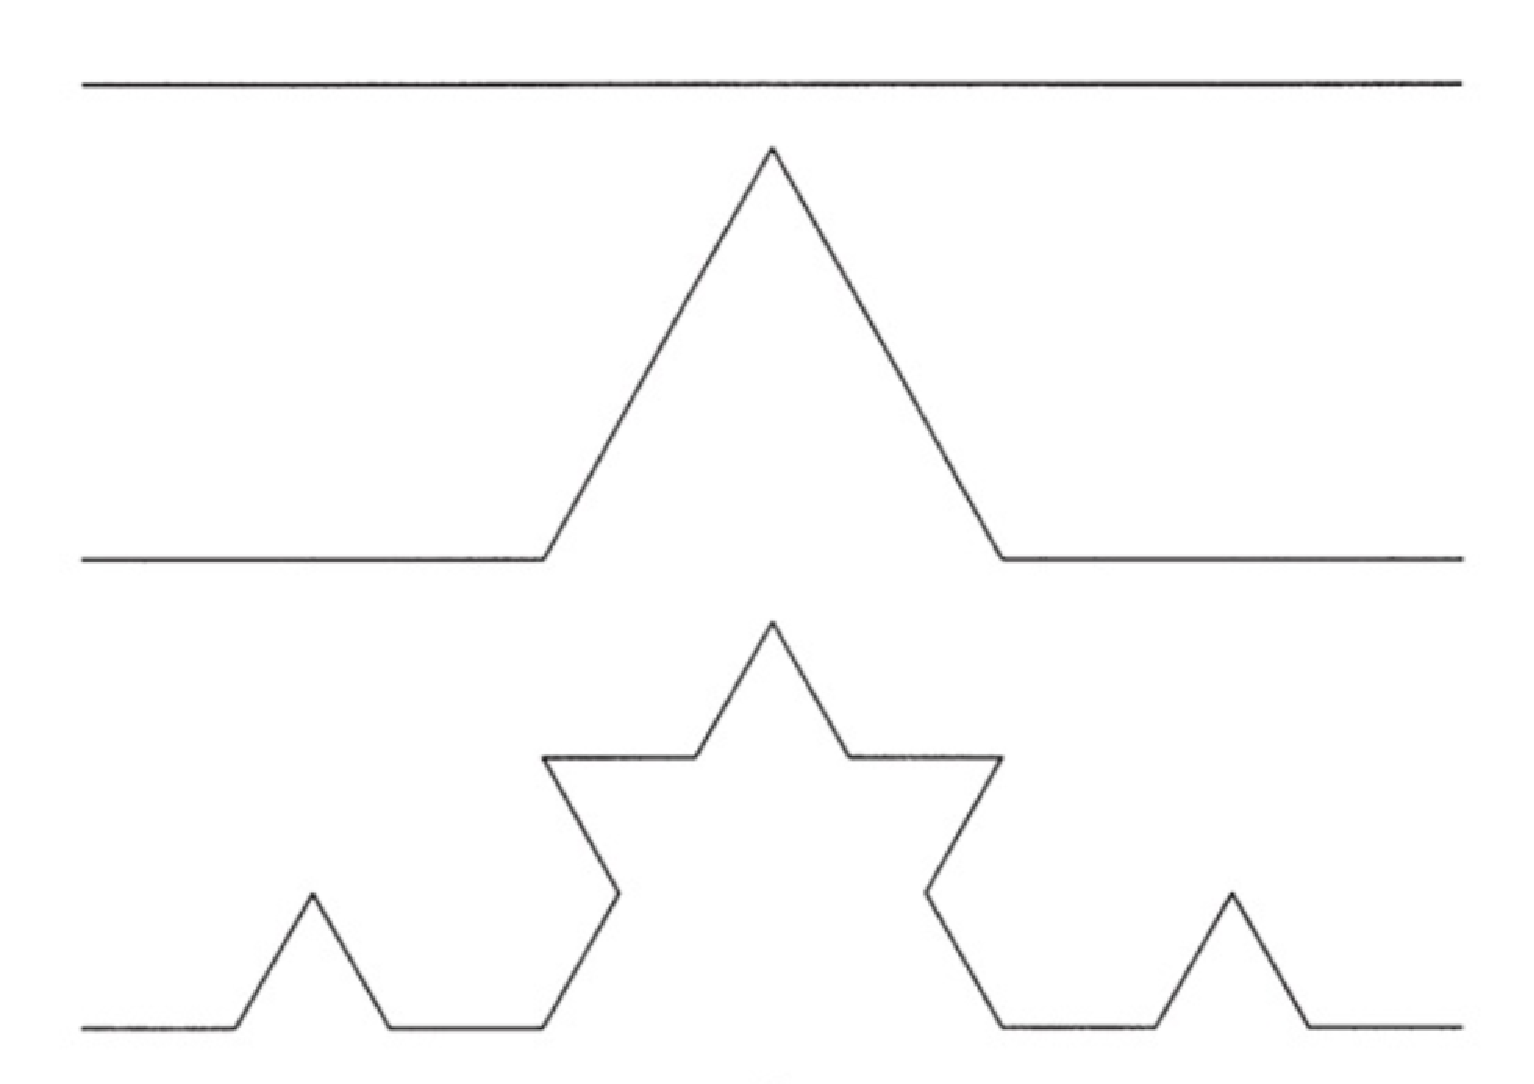
\includegraphics[width=0.8\textwidth]{figures/koch_curve.pdf}
    \caption{The Koch curve during three iterations \cite{strogatz:dynamics_chaos}.}
    \label{fig:koch_curve}
\end{figure}

The box counting method used in this thesis ressembles the method used in Equation (\ref{eq:similarityDimension}). But the scaling factor is not known, so the idea is to try to cover the fractal with a set of boxes of side length $\epsilon$. In the same way, the fractal dimension is defined as \cite{strogatz:dynamics_chaos}

\begin{equation}
    d = \lim_{\epsilon \to 0} \frac{\ln N(\epsilon)}{\ln 1 / \epsilon}
\end{equation}

Where $N(\epsilon)$ is the number of boxes with side length $\epsilon$ needed to cover the fractal.

In condensed matter physics, a lot of simulations operates on a lattice of spins, representing for example atoms in a grid. In 2001 an algorithm called the Worm algorithm was proposed \cite{Prokofev:first_worm_algorithm}. Instead of operating on individual spins, it generates spin configurations by `connecting' lattice sites together. This algorithm then generates a set of objects which have fractal like properties \cite{Duplantier:GeoHausdorff}.

The simplest such lattice is called the Ising lattice, where each spin can have one of two values. When the Worm algorithm is applied the resulting fractal in a two dimensional Ising lattice show similar dimension to a self avoiding walk. It is proposed to be a new such type of walk where `twisted loops' are allowed where the walk is allowed to cross itself, but still has elements of self-avoidance.

The XY model adds some complexity by allowing each spin to rotate around some axis. This complexity shows in the Worm algorithm by adding a direction and weight to the connection. So instead of connecting site $a$ and site $b$, it connects site $a$ \textit{to} site $b$ with the weight $w$. There has been some contesting results of the fractal dimension of spin configurations on a $3D$ XY lattice \cite{Prokofev:comment_on_hove_hausdorff_crit_fluct}\cite{Hove:hausdorff_crit_fluctuations} and this thesis attempts to add to that discussion. 















\chapter{Physics in extra dimensions}\label{ch:ExtraDimensions}
\section{Ising model}

The Ising model consists of discrete atomic spins $S$ that can be found in two states represented by the values $\{-1, 1\}$. This can be applied to a lattice where $S_i$ is the spin of lattice site $i$.

The energy of such a configuration is then given by the Hamiltonian

\begin{equation}
    H = - J \sum_{\langle ij \rangle} S_i S_j
\label{eq:isingmodelhamiltonian}
\end{equation}

Where $J$ is the bond strength in the lattice.

% TODO: Maybe add about the expansion of the correlation function
\subsection{Loop expansion}
\label{subsec:IsingLoopExpansion}

Let $K = \beta J$ where $\beta = 1/k_{\text{B}} T$. Then from Equation (\ref{eq:isingmodelhamiltonian})

\begin{equation}
    \beta E = - K \sum_{\langle ij \rangle} S_i S_j
\end{equation}

The partition function $Z$ can therefore be written as

\begin{equation}
    Z = \sum_{\text{all states}} e^{-\beta E} = \sum_{\text{all states}} e^{K \sum_{\langle ij \rangle} S_i S_j} = \sum_{\text{all states}} \Pi_{\langle ij \rangle} e^{K S_i S_j}
\label{Eq:partitionIsingWithoutExpansion}
\end{equation}

Since $S_i S_j = \pm 1$ Euler identities can be used to expand the exponential in Equation (\ref{Eq:partitionIsingWithoutExpansion}).

\begin{align*}
    e^{KS_i S_j} &= \frac{e^K + e^{-K}}{2} + S_i S_j \frac{e^K - e^{-K}}{2} \\
    &= \cosh (K) + S_i S_j \sinh(K) \\
    &= \{ T = \tanh(K) \} \\
    &= (1 + T S_i S_j) \cosh(K)
\end{align*}

In a $2D$ lattice with $N$ spins and periodic boundary conditions there are $2N$ bonds. Therefore the partition function is

\begin{align*}
    Z &= \sum_{\text{all states}} \Pi_{\langle ij \rangle} (1 + T S_i S_j) \cosh(K) \\
    &= \cosh^{2N} (K) \cdot 2^N \left ( 2^{-N} \sum_{\text{all states}} \Pi_{\langle ij \rangle} (1 + T S_i S_j) \right ) \\
    &= \cosh^{2N} (K) \cdot 2^N Z'
\end{align*}

Where

\begin{align*}
    Z' &= 2^{-N} \sum_{\text{all states}} \Pi_{\langle ij \rangle} (1 + T S_i S_j) \\
    &= 2^{-N} \sum_{S_1 = \pm 1} \sum_{S_2 = \pm 1} \ldots \sum_{S_N = \pm 1} \left ( 1 + T \sum_{l = 1} S_i S_j + T^2 \sum_{l = 2} (S_i S_j)(S_{i'} S_{j'}) + \ldots \right ) 
\end{align*}

Where the sums $\sum_{l=L}$ should be interpreted as the sum over all sets where the link length is $L$. Link length is the number of coupling terms $S_i S_j$ as can be seen in Figure (\ref{fig:LinkIsing}).

\begin{figure}[h!]
    \begin{subfigure}{.5\linewidth}
        \centering
        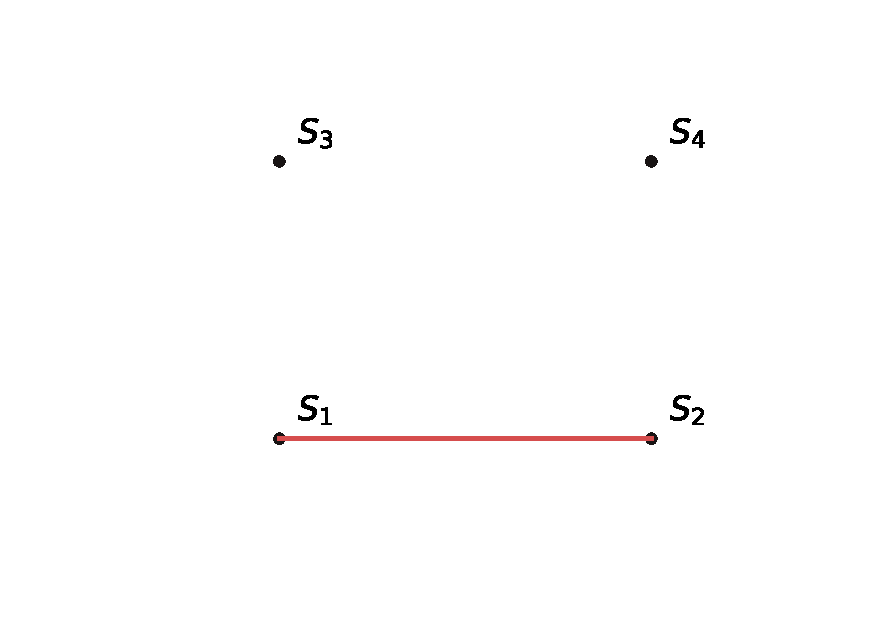
\includegraphics[width=\textwidth]{figures/ising_loop_one_link.pdf}
        \caption{$(S_1 S_2), \ L = 1$}
        \label{fig:oneLinkIsing}
    \end{subfigure}%
    \begin{subfigure}{.5\linewidth}
        \centering
        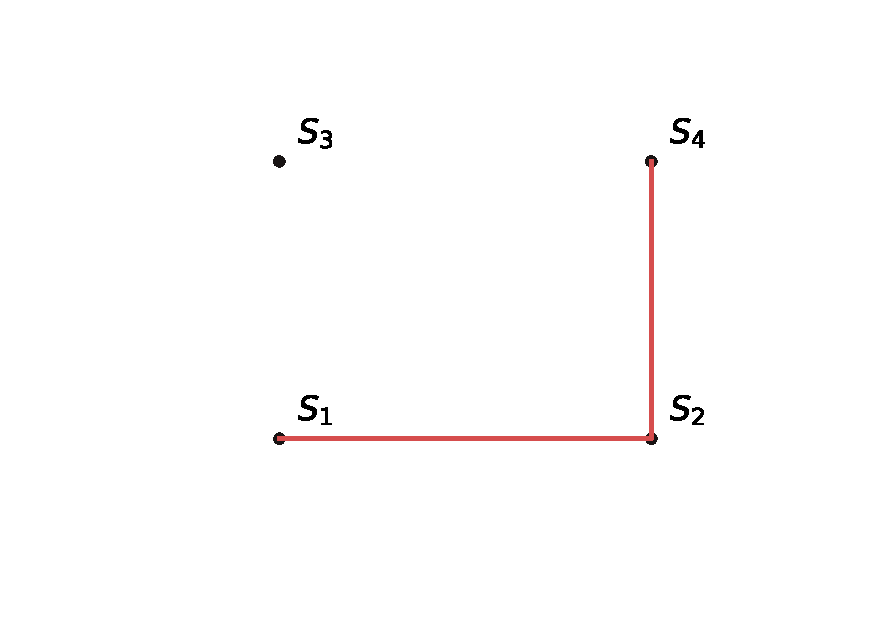
\includegraphics[width=\textwidth]{figures/ising_loop_two_link.pdf}
        \caption{$(S_1 S_2)(S_2 S_4), \ L = 2$}
        \label{fig:twoLinkIsing}
    \end{subfigure}\\[1ex]
    \begin{subfigure}{\linewidth}
        \centering
        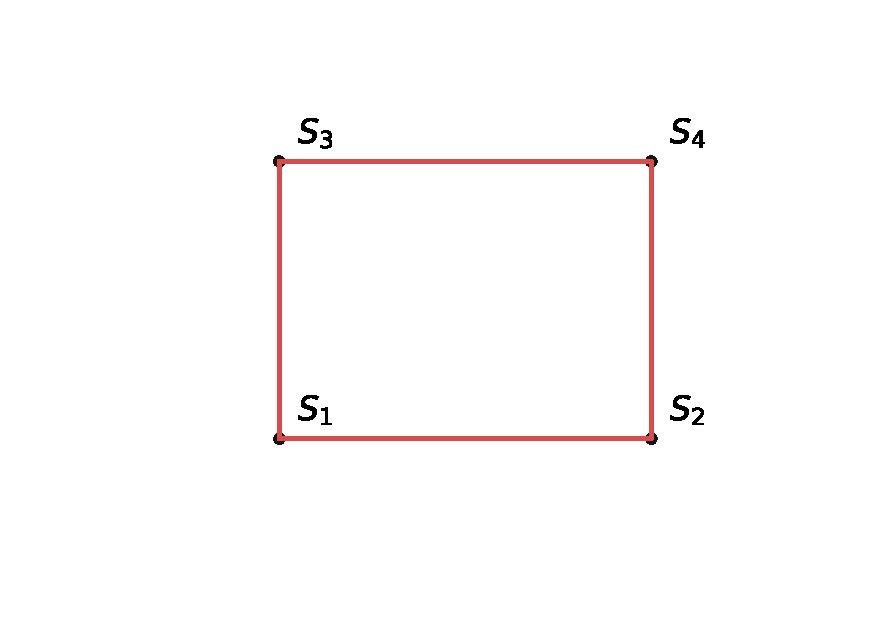
\includegraphics[width=.5\textwidth]{figures/ising_loop_four_link.pdf}
        \caption{$(S_1 S_2)(S_2 S_4)(S_4 S_3)(S_3 S_1), \ L = 4$}
    \label{fig:fourLinkIsing}
    \end{subfigure}
    \caption{Link structure of an Ising lattice where (a) and (b) are open while (c) is closed.}
    \label{fig:LinkIsing}
\end{figure}

Since $\sum_{S_i = \pm 1} S_i = 0$, only terms with an even number of $S_i$ are contributing to $Z'$. Call these terms closed, indicating that they represent a closed loop. The sum over all contributing terms gives a factor of $2^N$.

Rewriting $Z'$ in terms of loop lengths gives

\begin{equation}
    Z' = \sum_L g(L) T^L
\end{equation}

Where $g(L)$ is the number of loops with length $L$. Finally, the partition function can be written as

\begin{equation}
    Z = 2^N \cosh^{2N} (K) \sum_L g(L) T^L
\end{equation}

\subsection{Correlation Function}
\label{subsec:CorrelationFunction}

By the fluctuation-dissipation theorem the susceptibility can be written as \cite{Chaikin:PrincCondencedMatterPhysics}

\begin{equation}
    \chi = \frac{\beta}{N} \sum_{ij} G_{ij}
\end{equation}

Where $G_{ij} = \langle S_i S_j \rangle - \langle S_i \rangle^2$ is the connected correlation function between two lattice points $i$ and $j$.

In the high-temperature expansion the term $\langle S_i \rangle^2$ goes to zero. So for a $2D$ Ising model

\begin{align}
    G_{ij} &= \frac{1}{Z} \sum_{\text{all states}} S_i S_j e^{-\beta E} \\
    &= \left \{ \text{See Section \ref{subsec:IsingLoopExpansion}} \right \} \\
    &= \frac{1}{Z} \cosh^{2N} (K) \sum_{\text{all states}} S_i S_j \Pi_{\langle ij \rangle} (1 + \tanh(K) S_i S_j)
\end{align}

So the acceptance probability (See Section \ref{sec:MetropolisAlgorithm}) is \cite{Walter:IntroToMC}

\begin{equation}
A_{ab} = \left\{
\begin{array}{ll}
      \min \left (1, \tanh(K)\right), \ \text{To create a link between $a$ and $b$.} \\
      \min \left (1, \frac{1}{\tanh(K)} \right), \ \text{To remove a link between $a$ and $b$.}
\end{array} 
\right. 
\end{equation}



\section{$n$-vector model}
\label{sec:nVector}

The $n$-vector model describes a classical system of $n$-dimensional classical spins $s_i$ of unit length interacting on a lattice. It is a generalization of the Ising model where each spin can have a continuous set of values. The Hamiltonian is then

\begin{equation}
    H = -J\sum_{\langle ij \rangle} s_i \cdot s_j
\end{equation}

where $J$ is the bond strength and $\langle ij \rangle$ refers to a nearest neighbour interaction.

\section{XY model}
\label{sec:XYModel}

A special case of the $n$-vector model is the XY model when $n = 2$. Here the spins are two dimensional rotors as $s_i = (\cos \theta_i, \  \sin \theta_i)$. This yields the Hamiltonian

\begin{equation}
    H = - J \sum_{\langle ij \rangle} \cos(\theta_i - \theta_j)
\label{eq:xymodel}
\end{equation}

The partition function is therefore

\begin{equation}
    Z = \prod_i \int \frac{\mathrm d \theta_i}{2 \pi} e^{-\beta H} = \prod_i \int \frac{\mathrm d \theta_i}{2 \pi} e^{K \sum_{\langle ij \rangle} \cos(\theta_i - \theta_j)}
\label{eq:xypart1}
\end{equation}

where $K = J \beta$.

\subsection{Loop expansion}
\label{subsec:XYLoopexp}

Since equation (\ref{eq:xypart1}) is invariant under the transformation $\theta_i - \theta_j \rightarrow \theta_i - \theta_j + 2 \pi n$, $n \in \mathbb{Z}$, it can be expanded using the identity

\begin{equation}
    e^{\alpha \cos \beta} = \sum_{\gamma = -\infty}^{\infty} I_\gamma ( \alpha ) e^{i \gamma \beta}
\end{equation}

where $I_\gamma(\alpha)$ is the modified Bessel function. Using that $e^{\sum_i x_i} = \prod_i e^{x_i}$

\begin{align}
    Z &= \prod_i \int \frac{\mathrm d \theta_i}{2 \pi} \sum_{J_{\langle ij \rangle} = -\infty}^{\infty} \prod_{b = \langle ij \rangle} I_{J_{\langle ij \rangle}} ( K ) e^{i J_{\langle ij \rangle} (\theta_i - \theta_j)} \\
\label{eq:xypart2}
% 
    &=  \prod_i \sum_{J_b} \left ( \int \frac{\mathrm d \theta_i}{2 \pi} e^{i N_i (\theta_i - \theta_j)} \right ) \left ( \prod_b I_{J_b} \right ) 
\end{align}

Where in the last step, $\prod_{\langle ij \rangle} e^{iJ_{\langle ij \rangle} (\theta_i - \theta_j)} = e^{iN_i (\theta_i - \theta_j)}$. $N_i$ is therefore the sum of $J$ for the nearest neighbours of site $i$. Noting that

\begin{equation}
    \int \frac{\mathrm d \theta_i}{2 \pi} e^{i N_i (\theta_i - \theta_j)} = C \delta_{N_i 0}
\end{equation}

leads to the conclusion that the sum of incoming and outgoing flux $J$ into a site $i$ must be zero, in other words, the configurations are divergence free. This in turn means that a configuration of the system must contain closed loops of flux $J$.

% NOTE: Explanation to the last sentence; take one site i and impose that it has to be divergence free (some flux out, same flux in). Then impose the same thing on its neighbour. The flux coming out of i must flow into the neighbour. Repeating this process over the whole lattice will give closed loops.

\subsection{Winding number}
\label{subsec:XYWindingNum}

In the ground state all the spins are aligned, while at higher energy states, the spins are pointed in random directions as can be seen in Figure (\ref{fig:xygroundhigher}).

\begin{figure}[h!]
\centering
    \begin{subfigure}{.4\textwidth}
        \centering
        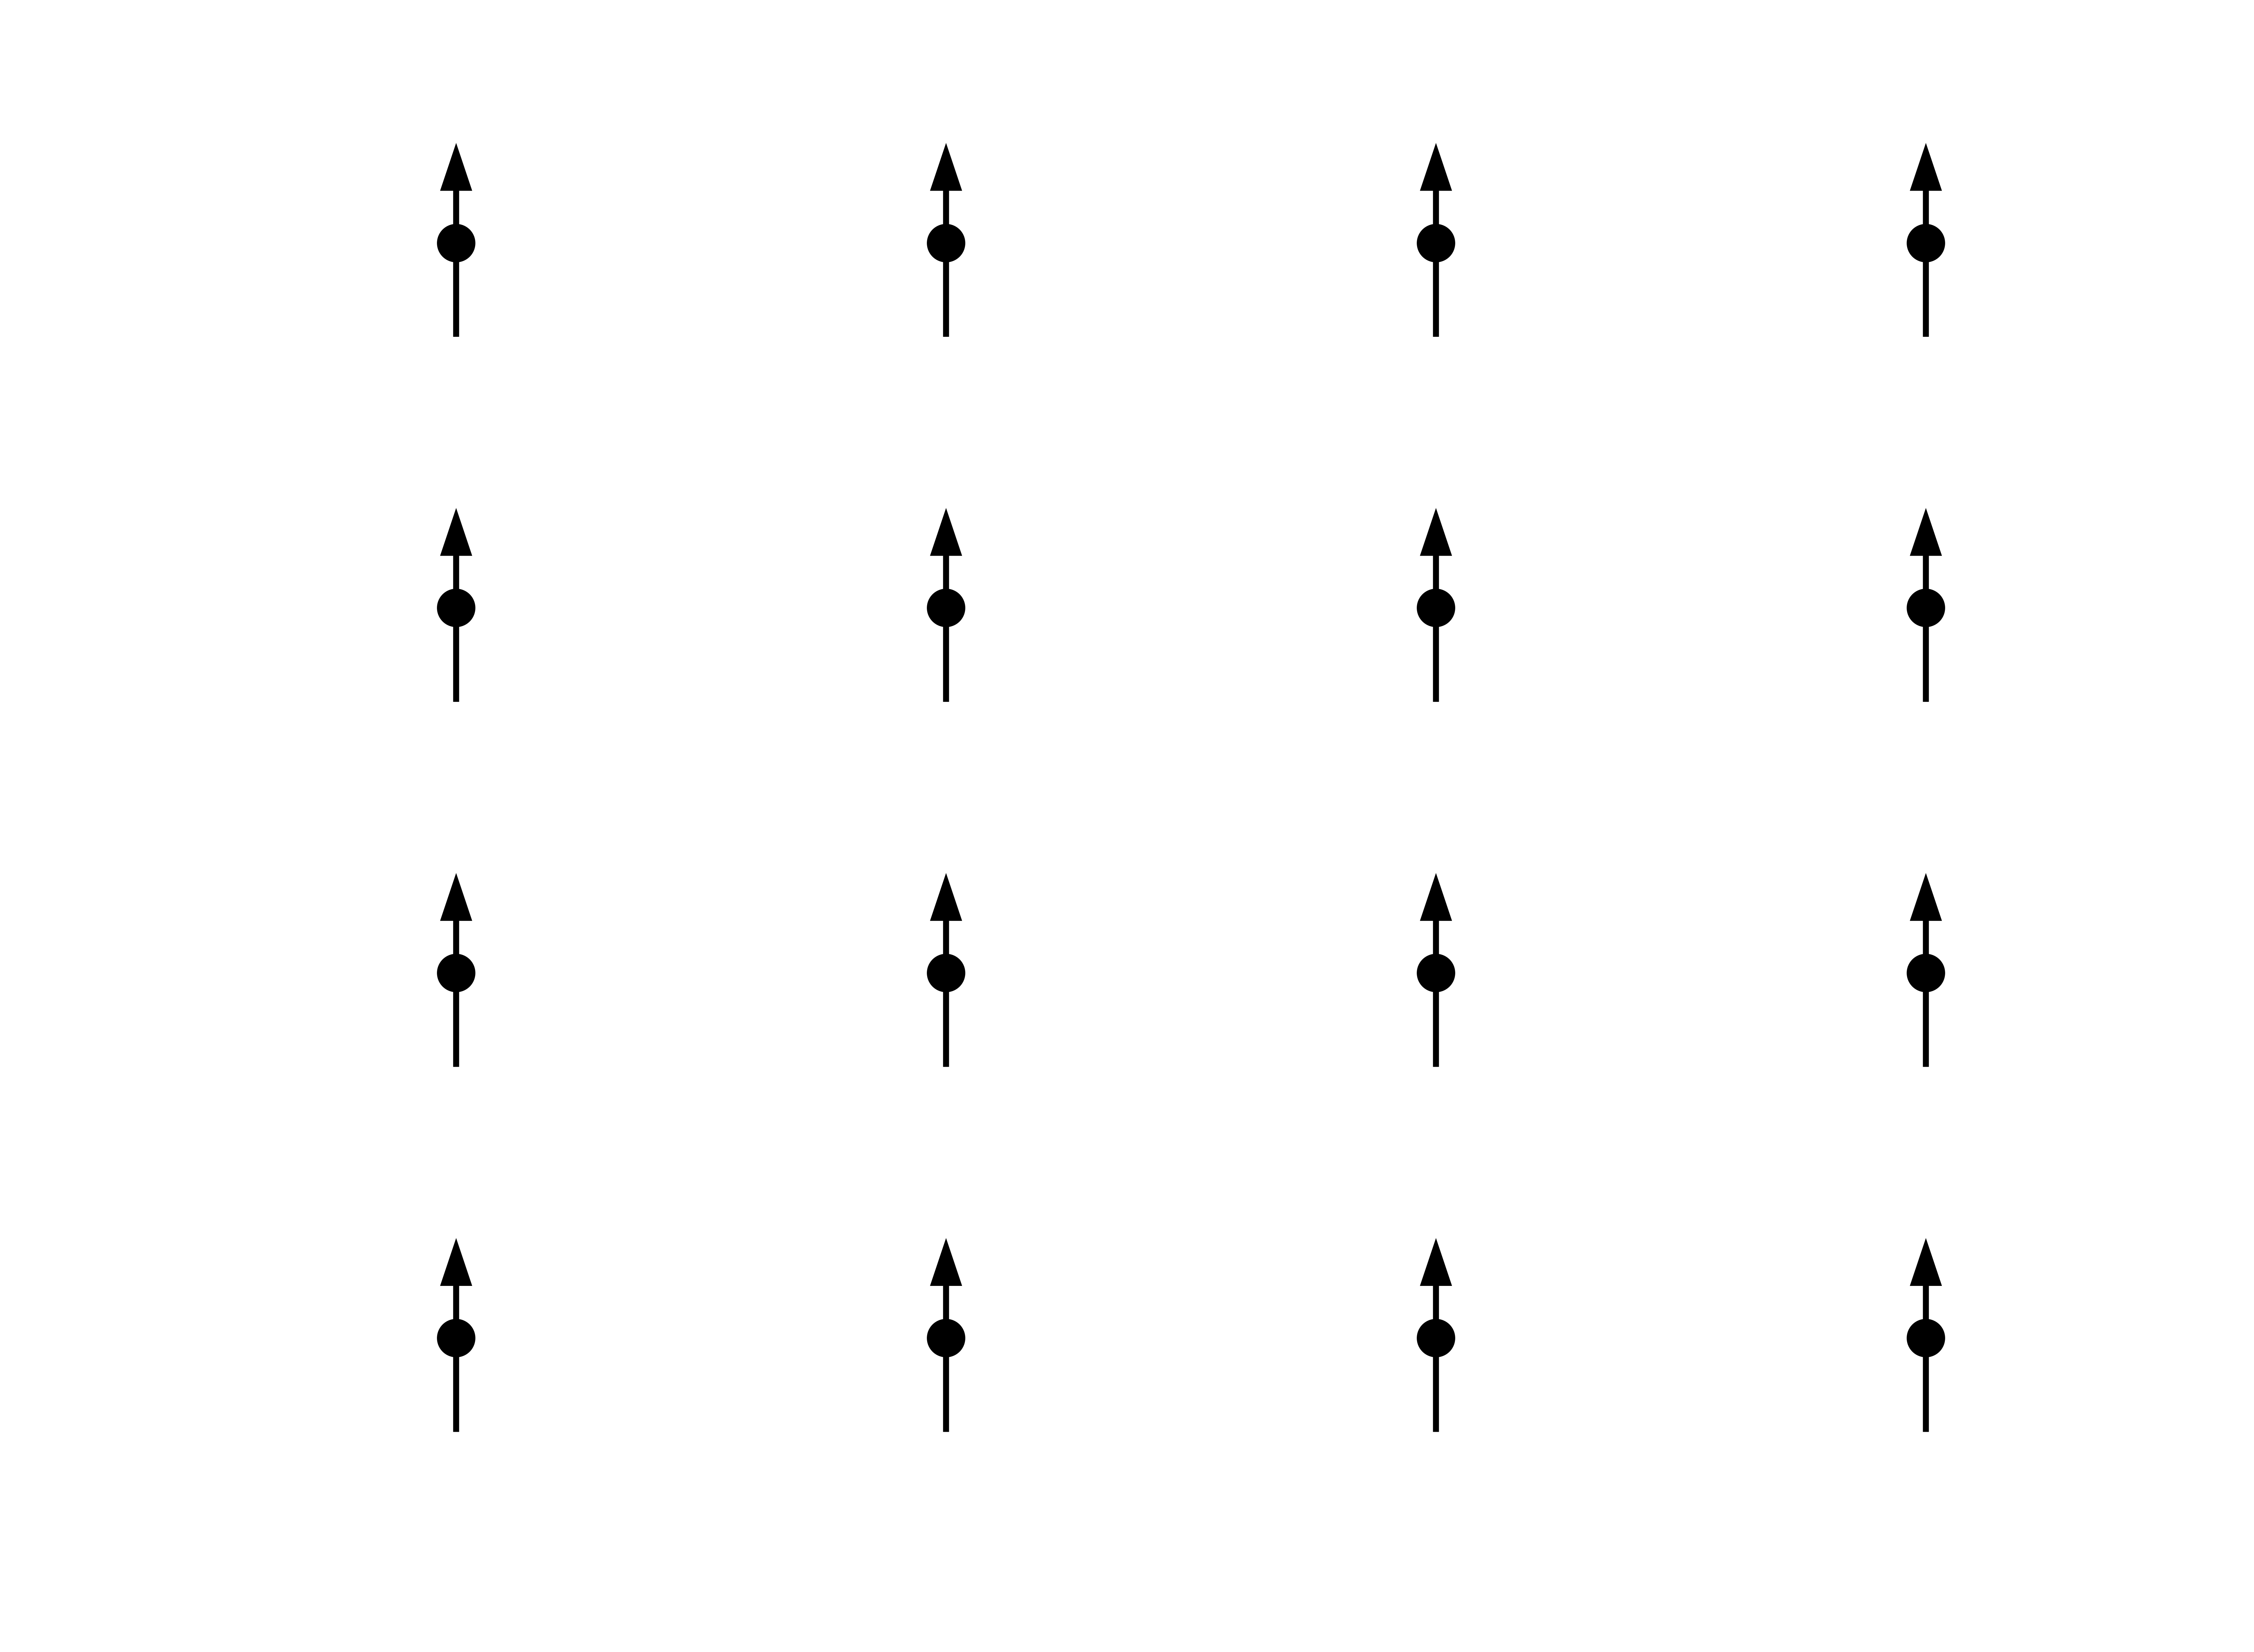
\includegraphics[width=\linewidth]{figures/noPhaseShift.pdf}
        \caption{Ground state}
        \label{fig:xyground}
    \end{subfigure}
    \begin{subfigure}{.4\textwidth}
        \centering
        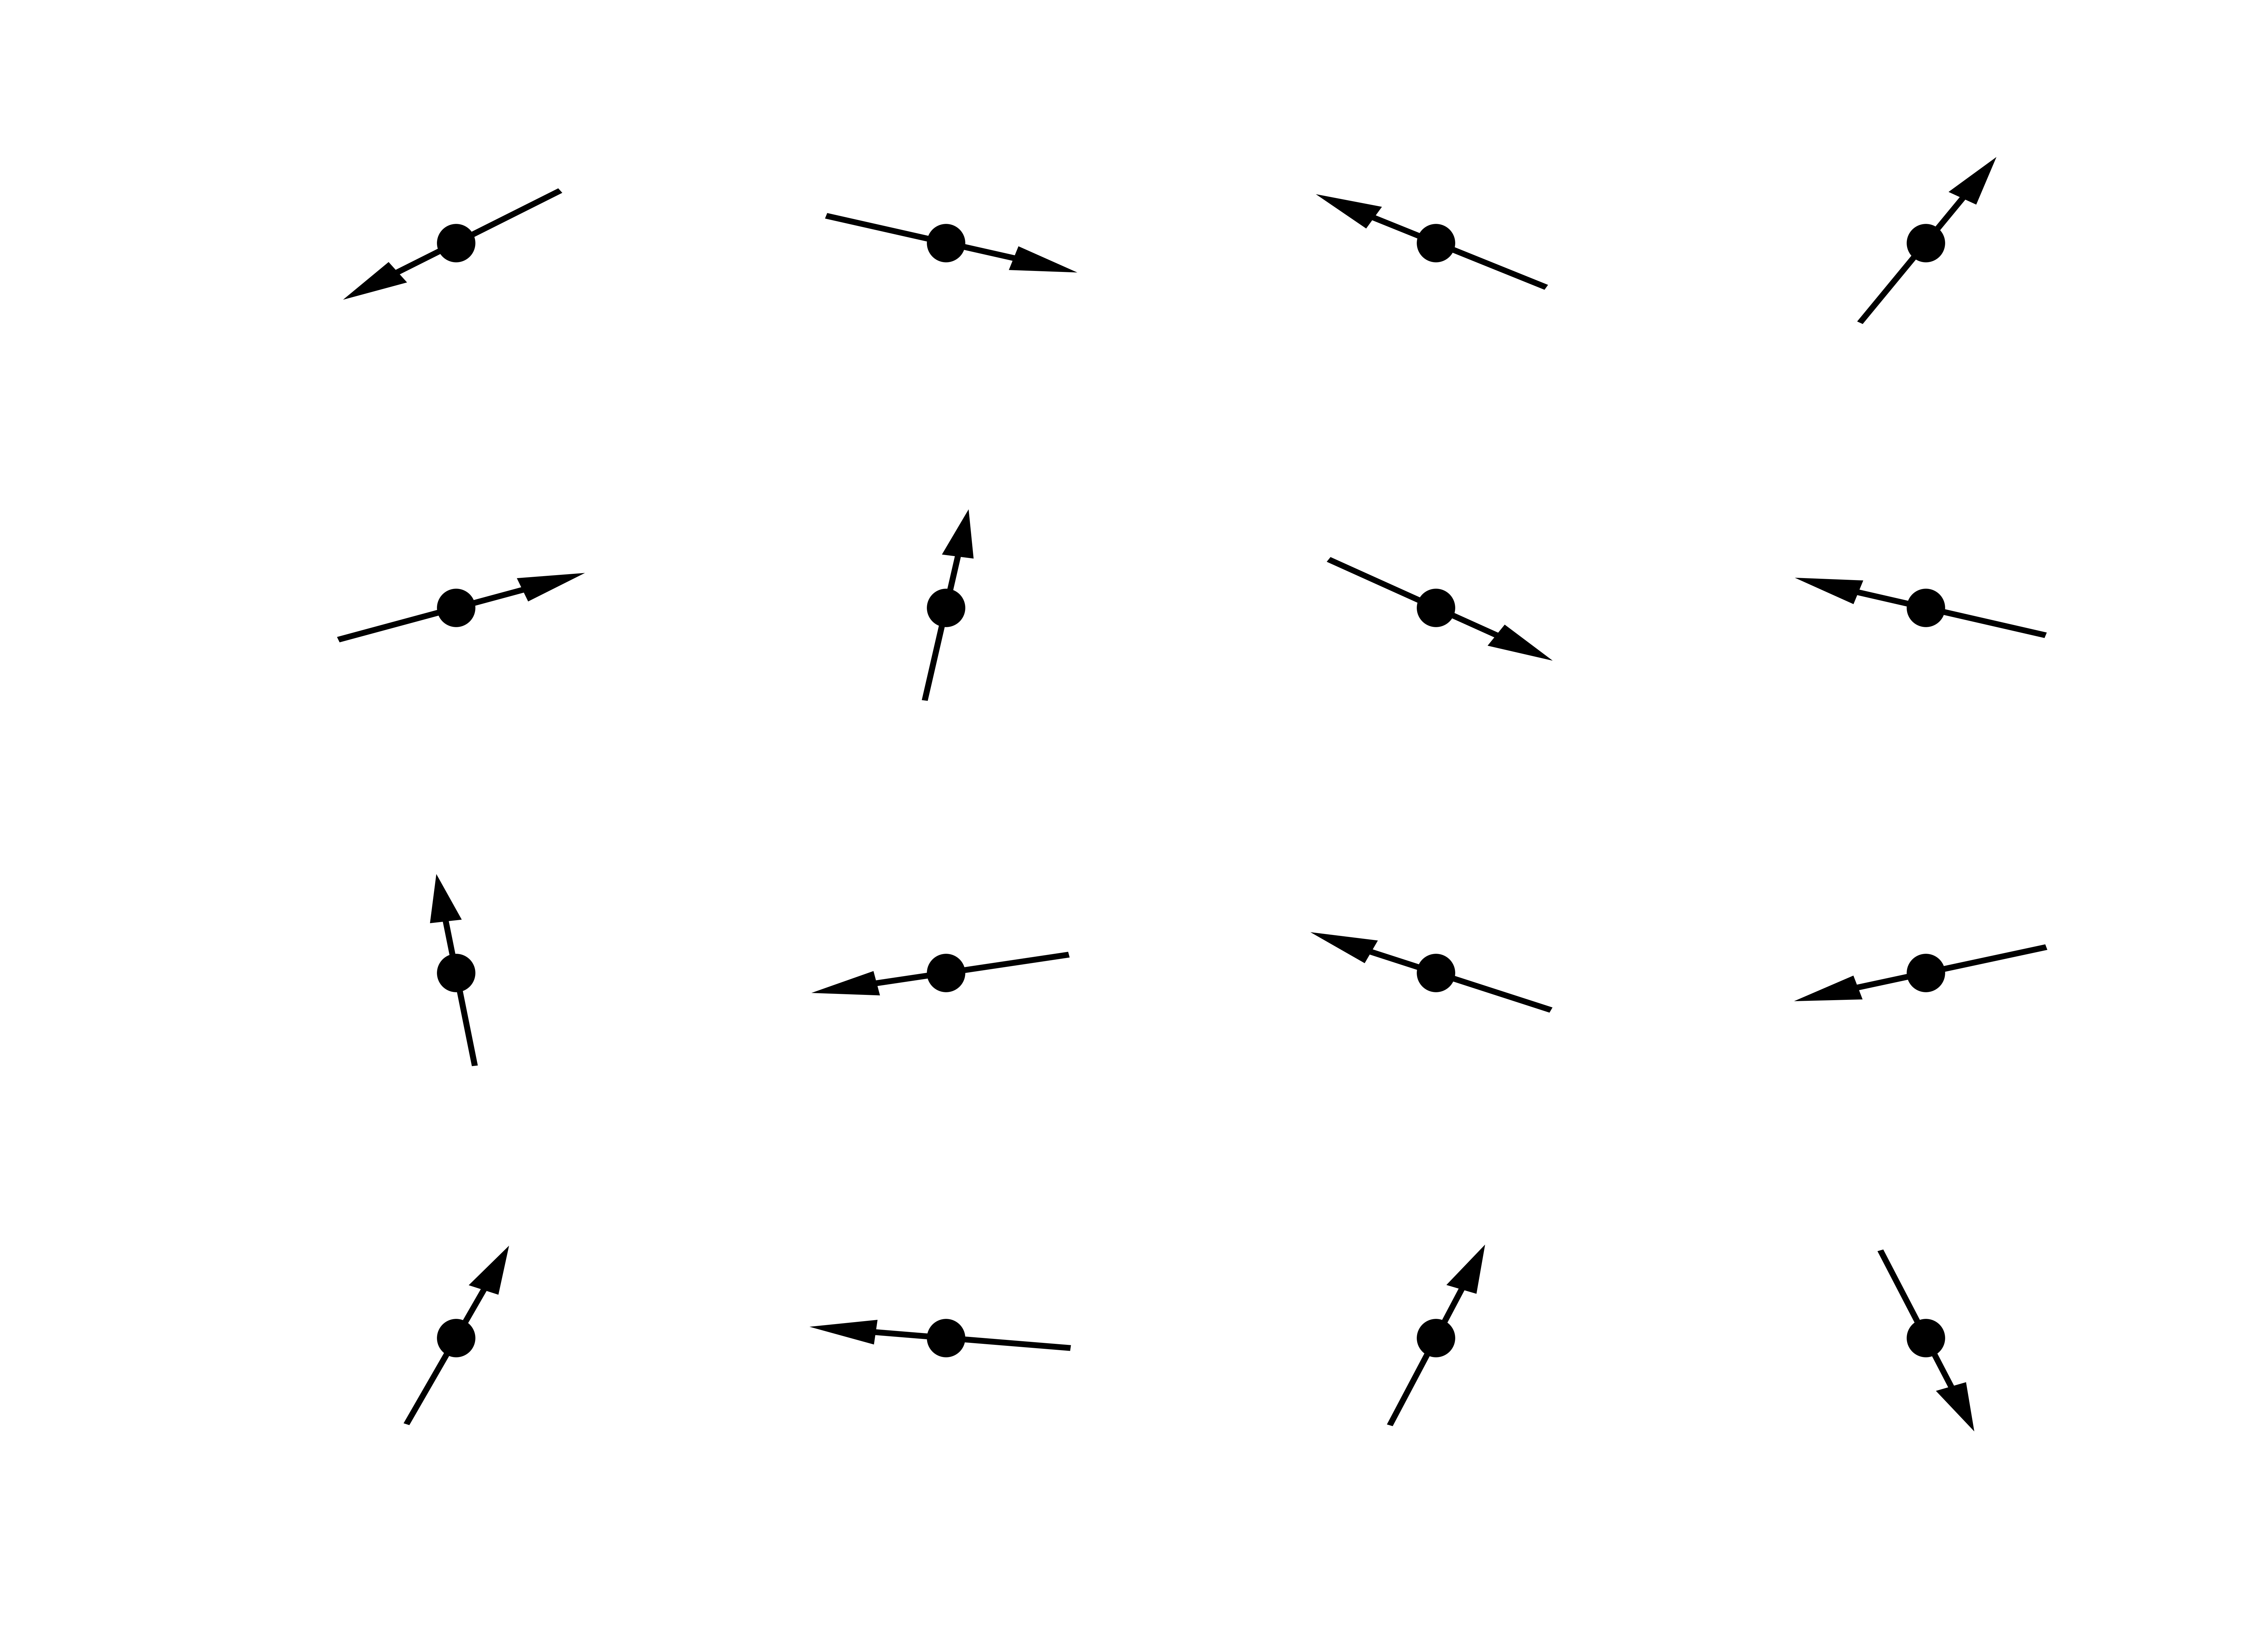
\includegraphics[width=\linewidth]{figures/randomAngle.pdf}
        \caption{Higher energy state}
        \label{fig:xyhigher}
    \end{subfigure}
    \caption{Energy states for XY model}
\label{fig:xygroundhigher}
\end{figure}

Therefore, making a constant phase shift $\Phi_\mu = \frac{A}{L}$ of $\theta_i - \theta_j$ in the $\mu$ direction would change the energy drastically for the ground state while, on a statistical average, not change the higher states energy at all (see Figure (\ref{fig:xyphaseshift})).

\begin{figure}[h!]
\centering
    \begin{subfigure}{.4\textwidth}
        \centering
        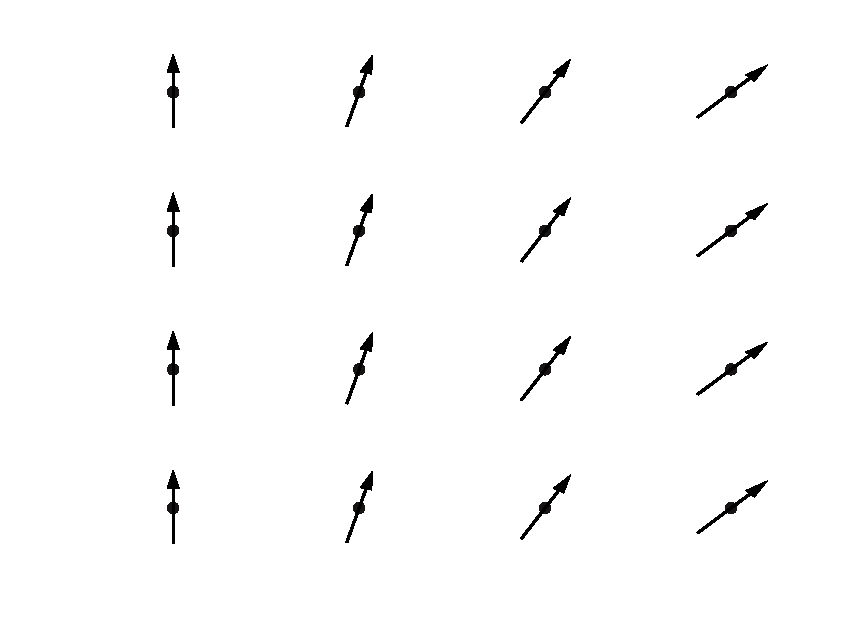
\includegraphics[width=\linewidth]{figures/PhaseShift.pdf}
        \caption{Ground state}
        \label{fig:xyground}
    \end{subfigure}
    \begin{subfigure}{.4\textwidth}
        \centering
        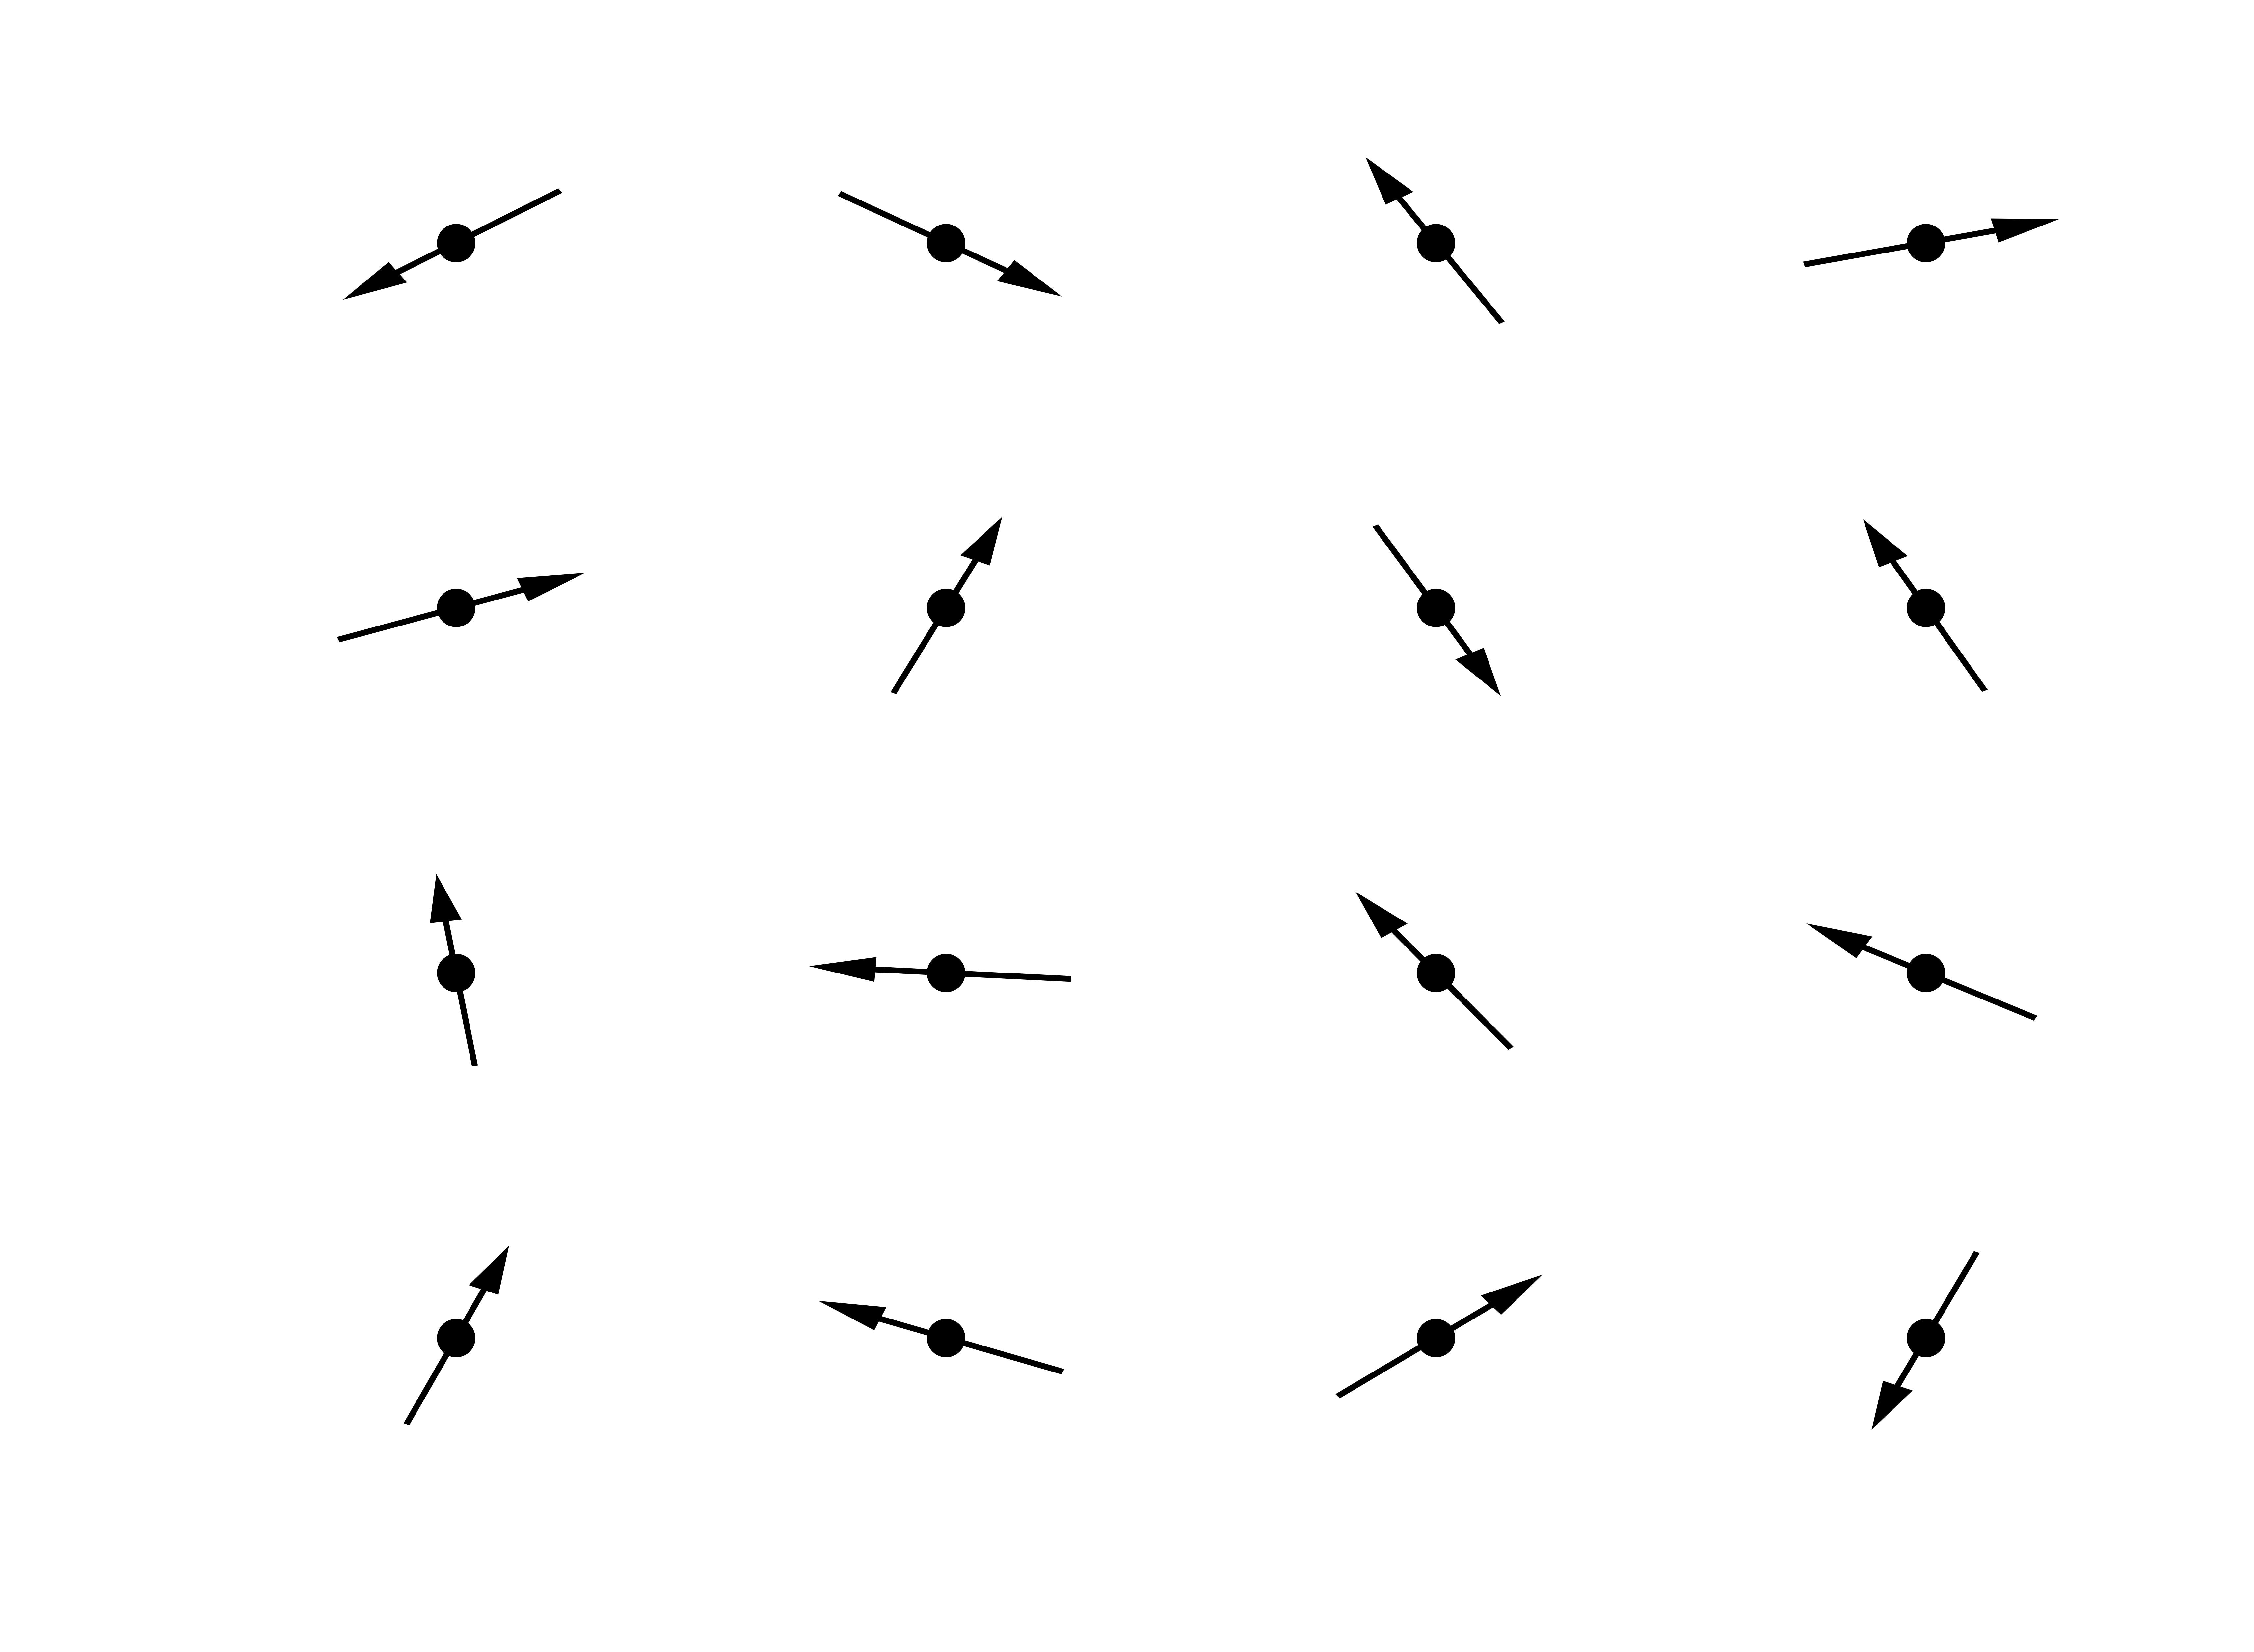
\includegraphics[width=\linewidth]{figures/randomPhaseShift.pdf}
        \caption{Higher energy state}
        \label{fig:xyhigher}
    \end{subfigure}
    \caption{A phase shift for $\mu = x$}
\label{fig:xyphaseshift}
\end{figure}

The free energy change $\Delta F$ for such a shift is

\begin{equation}
    \Delta F = L^d \cdot \frac{1}{2} \rho_s \left( \frac{A}{L} \right)^2 \Rightarrow \rho_s = \lim_{A \to 0} L^{2 - d}\frac{\partial^2 \Delta F}{\partial A^2}
\end{equation}

where $d$ is the dimension and $\rho_s$ is the superfluid density which is zero for a high energy state. The free energy is

\begin{equation}
F = - T \ln(Z) \Rightarrow F'' = T \left(\left(\frac{Z'}{Z}\right) - \left( \frac{Z''}{Z} \right)^2 \right)
\label{eq:xyfreeenergy}
\end{equation}

where $F' = \partial F / \partial A$. Examining $Z$ from (\ref{eq:xypart2}) with the added shift

\begin{align}
    Z &= \prod_i \int \frac{\mathrm d \theta_i}{2 \pi} \sum_{J_{\langle ij \rangle} = -\infty}^{\infty} \prod_{b = \langle ij \rangle} I_{J_{\langle ij \rangle}} ( K ) e^{i J_{\langle ij \rangle} (\theta_i - \theta_j + \Phi_\mu)} \\
%
    & = \prod_i \sum_{J_b} \left ( \int \frac{\mathrm d \theta_i}{2 \pi} e^{i N_i (\theta_i - \theta_j)} \right ) \left ( \prod_b I_{J_b} \right ) \cdot e^{i A \frac{1}{L} \sum_i J_{i, i+\mu}} \\
\label{eq:xypart3}
\end{align}

where in the last step

\begin{align}
    \prod_i \left (\prod_{\langle ij \rangle} e^{i J_{\langle ij \rangle} \Phi_\mu} \right) &= \\
%
    \left\{ \text{$\Phi_\mu \neq 0$ only for neighbours in the $\mu$ direction} \right \} &= \\
%
    \prod_i \left ( e^{iJ_{i, i+\mu} \Phi_\mu} \right ) &= \\
%
    e^{iA \frac{1}{L} \sum_i J_{i, i+\mu}}
\end{align}

Introduce the winding number in the $\mu$ direction as

\begin{equation}
    W_\mu = \frac{1}{L} \sum_i J_{i, i+\mu}
\label{eq:defwinding}
\end{equation}

Intuitively, this describes the net flux in the $\mu$-direction. Given a loop within the bounds of the lattice, the winding number is always zero. This is since an equal amount of flux in $+\mu$ as in $-\mu$ is needed to form a loop. However, this is not the case for a percolating cluster going, for example, from $-\mu$ to $+\mu$ connecting with periodic boundary conditions. For such a `winding' cluster, the winding number will be $+1$. An example can be seen in figure (\ref{fig:fluxpercolation}).

\begin{figure}[h!]
    \centering
        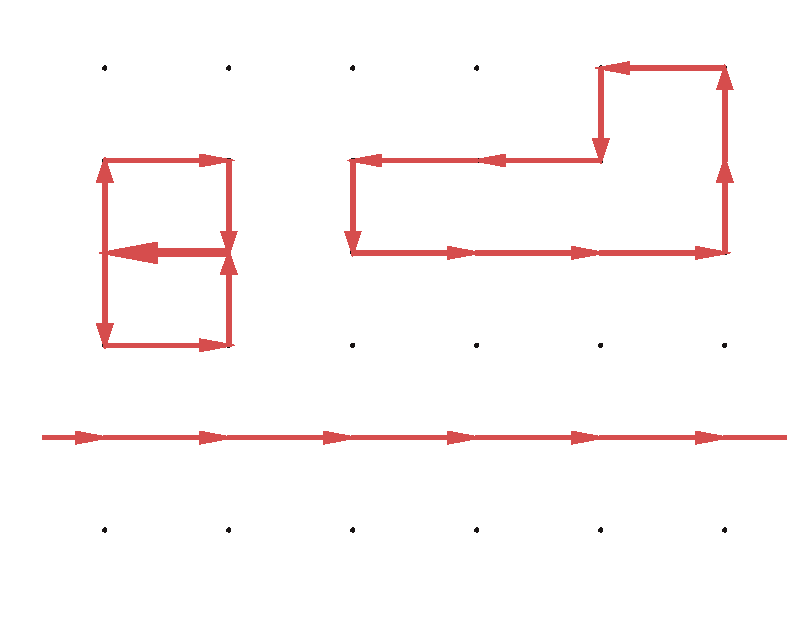
\includegraphics[width=0.8\textwidth]{figures/percolatingFlux.pdf}
    \caption{Three flux clusters on a square lattice. One percolating cluster with $W_x = +1$. The size of each arrow corresponds to the number of flux quanta between two sites.}
    \label{fig:fluxpercolation}
\end{figure}

Using the definition (\ref{eq:defwinding}) for the winding number in the partition function in equation (\ref{eq:xypart3}) yields

\begin{align}
    Z &= \sum_{J_b} \left ( \prod_b I_{J_b} \right ) \prod_i \left ( \int \frac{\mathrm d \theta_i}{2 \pi} e^{i N_i (\theta_i - \theta_j)} \right ) \cdot e^{i A W_\mu} \\
    &= \sum_{J_b, \ N_i = 0} Z_0 \cdot e^{i A W_\mu} \\
    &= \sum_{W_\mu} Z_0 \cdot e^{i A W_\mu}
\end{align}

Using this result in equation (\ref{eq:xyfreeenergy})

\begin{align}
    \frac{\partial^2 F}{\partial A^2} &= T \left ( \left ( \frac{\sum_{W_\mu} (i W_\mu) Z_0 e^{iAW_\mu}}{\sum_{W_\mu} Z_0 e^{iAW_\mu}} \right )^2 - \frac{\sum_{W_\mu} (- W_\mu^2) Z_0 e^{iAW_\mu}}{\sum_{W_\mu} Z_0 e^{iAW_\mu}} \right ) \\
%
    &= T \left ( -\langle W_\mu \rangle^2 + \langle W_\mu^2 \rangle \right ) \\
%
    &= T \langle W_\mu^2 \rangle
\end{align}

Where $\langle W_\mu \rangle = 0$ since there is an equal chance of percolating from $-\mu$ to $\mu$ as the other way around.

The superfluid density can finally be determined as

\begin{equation}
    \rho_s = L^{2 - d} T \langle W_\mu^2 \rangle 
\end{equation}

\subsection{Villain approximation}
\label{subsec:villainApprox}


The Villain model the Hamiltonian has the form \cite{Villain:VillainOriginalPaper}

\begin{equation}    
    H = \sum_{ij} V_{ij}( \theta_i - \theta_j) + \sum_i U(\theta_i)
\end{equation}

By taking

\begin{align}
    V_{ij}( \theta_i - \theta_j) &= -J \cos ( \theta_i - \theta_j) \\
    U( \theta_i ) &= 0
\end{align}

The XY model in Equation (\ref{eq:xymodel}) is recovered.

The approximation then made by Villain was to replace the magnetic Hamiltonian by an approximate one \cite{Villain:VillainOriginalPaper}.

Through a series of transformations the energy in this approximation can be written as \cite{Jos:VillainExtended}

\begin{equation}
    E = \frac{1}{2} \sum_i J_i^2
\end{equation}

Where $J_i^2$ is the flux from site $i$.

The acceptance probability (See Section \ref{sec:MetropolisAlgorithm}) is therefore

\begin{align}
    A_{ab} &= \min \left ( 1, e^{-\Delta E} \right ) \\
    &= \min \left ( 1, e^{-\frac{1}{2} \Delta J_{ab}^2} \right )
\end{align}

Where $J_{ab}$ is the link between site $a$ and $b$.

\subsection{Energy Scaling}
\label{subsec:xyenergyScaling}

The scaling behaviour of the heat capacity is% TODO: CITE HERE

\begin{equation}
    C = \frac{e}{t} = \tilde a t^{-\alpha} + \tilde b
\end{equation}

where $t = |T - T_c|$, $\alpha = -0.01$, and $\tilde a, \ \tilde b$ are some constants.

Therefore, the energy per site, $e$ is

\begin{equation}
    e = a t^{1 - \alpha} + b
\end{equation}

And the total energy

\begin{equation}
    E = L^d ( a t^{1 - \alpha} + b ) \propto L^3, \ \text{at $T = T_c$}
\end{equation}

where $d$ is the dimension of the sample. This scaling behaviour for the total energy can be seen in Figure (\ref{fig:results_energyxy}) for $d = 3$.

\section{Hausdorff dimension}
\label{sec:hausdorffdimension}

% TODO: Write about Hausdorff dimension from the book on Telegram

Let $X$ be a metric space, $\alpha$ be some positive real number, then the $\alpha$-Hausdorff measure of a subset $A \subset X$ is defined as \cite{Heinonen:HausdorffDimMath}

\begin{equation}
    \mathcal{H}^{\delta}_\alpha (A) = \inf \left \{ \sum_{B \in \mathcal{B}} \left ( \text{diam}(B) \right)^\alpha \right \}
\end{equation}

Where $\mathcal{B}$ is a cover of $A$ of closed balls with diameter no larger than $\delta$.

Taking the limit where $\delta \to 0$, the number of possible covers decreases. Since the limit is bounded from below, the limit exists \cite{Rudin:PrincMathAnalysis} and

\begin{equation}
    \lim_{\delta \to 0} \mathcal{H}^{\delta}_{\alpha} (A) = \mathcal{H}_\alpha (A) \in [0, \infty )
\label{eq:hausdorffmeasure}
\end{equation}

Examining Equation (\ref{eq:hausdorffmeasure}) gives

\begin{align}
    \lim_{\delta \to 0} \mathcal{H}^{\delta}_{\alpha} (A) &= \lim_{\delta \to 0} \inf \left \{ \sum_{B \in \mathcal{B}} \left ( \text{diam}(B) \right)^\alpha \right \} \\
%
    &\leq \lim_{\delta \to 0} \inf \left \{ \sum_{B \in \mathcal{B}} \delta^\alpha \right \} \\
%
    &= \lim_{\delta \to 0} \inf \left \{ N_{\delta}^A \delta^\alpha \right \}
\end{align}

Where $N_{\delta}^A$ is the number of balls with diameter $\delta$ that can cover $A$. Though not a proof, one can intuitively say that if for some $\alpha > 0$ the limit is finite, then $\mathcal{H}_{\alpha'} = 0$ for each $\alpha' > \alpha$. Therefore the number

\begin{equation}
    \text{dim}_H (A) = \inf \{ \alpha > 0 : \mathcal{H}_\alpha (A) = 0 \}
\end{equation}

exists and is called the Hausdorff dimension of $A$ \cite{Heinonen:HausdorffDimMath}.


\section{Box dimension}
\label{sec:boxdimension}

Given some subset $A$ of a metric space $X$, let $N(\epsilon)$ be the number of boxes with side length $\epsilon$ needed to cover $A$. Then the box dimension $d$ of $A$ is defined as \cite{strogatz:dynamics_chaos}

\begin{equation}
    d = \lim_{\epsilon \to 0} \frac{\ln N(\epsilon)}{\ln 1 / \epsilon}
\end{equation}

If the limit exists.

For intuition it helps to look at some examples. If $A$ is a smooth line of length $l$, then the number of boxes needed to cover $A$ scales as

\begin{equation}
    N_l(\epsilon) \propto \frac{L}{\epsilon}
\end{equation}

While for some two dimensional region with area $\Lambda$ the boxes needed is

\begin{equation}
    N_{\Lambda}(\epsilon) \propto \frac{\Lambda}{\epsilon^2}
\end{equation}

Such that for a $d$-dimensional subset $A$, the boxes needed will scale as

\begin{equation}
    N (\epsilon) \propto \frac{1}{\epsilon^d} \Rightarrow d = \frac{\ln N(\epsilon)}{\ln 1 / \epsilon}
\end{equation}

Note that the box dimension and the Hausdorff dimension coincides for fractals that satisfy the open set condition \cite{Falconer:RelHausdorffBox}.

The open set condition says that for a sequence of contractions $c_1, c_2, ..., c_m$ exists a nonempty open set $V$ such that \cite{Bandt:OSC}

\begin{equation}
    \cup_{i = 1}^m c_i(V) \subset V, \ \text{and} \ c_i(V) \cap c_j(V) = \emptyset \ \text{for} \ i \neq j
\end{equation}

Intuitively, this means that the images $c_i(V)$ do not overlap `too much'.

\subsection{Scaling Dimension}
\label{subsec:ScalingDimension}

Another way of determining the Hausdorff dimension is to consider a scaling system \cite{Camarda:MethodsDetermineHausdorff}. The scaling behaviour of the largest cluster should then follow

\begin{equation}
    N = L^{D_H}
\end{equation}

Where $N$ is the number of links in the largest cluster, $L$ is the linear system length and $D_H$ is the Hausdorff dimension.

This scaling relation can be seen in Figure (\ref{fig:results_maxloopdimension}).




\chapter{Dark matter}\label{ch:DarkMatter}
\section{Monte Carlo Simulations}
\label{sec:MonteCarloSims}



\section{Ergodicity}
\label{sec:Ergodicity}

\section{Detailed Balance}
\label{sec:DetailedBalance}

\section{Worm Algorithm}
\label{sec:WormAlgorithm}

\section{Testing}
\label{sec:Testing}

Testing is an essential part of writing a simulation. The correctness of the code ensures that the physical model is aptly described. To facilitate the development, a number of coding practices were applied, such as unit testing (Section \ref{sec:UnitTesting}) and regression testing (Section \ref{sec:RegressionTesting}). The tests for the prototypes were written in the Python standard library utility \textit{unittest}, and those for the main simulation used the C++ framework \textit{Catch2}.

\subsection{Unit Testing}
\label{sec:UnitTesting}

Unit testing refers to the practice of isolating a `unit' of code and testing its correctness. A unit can be any small piece of code with an expected behaviour.

This was done by manually calculating the expected output of some code, given some input, and ensuring that the piece of code produced an equivalent result.

The parts of the simulation using a pseudorandom number generator were tested by randomly selecting a set of seeds on which the tests were run upon. The correctness is then assumed from this subset of possible inputs.

When multiple unit tests are tested together, it is called integration testing. This assumes that each unit is correct by itself, and it was used to more closely ressemble the actual simulation.

\subsection{Regression Testing}
\label{sec:RegressionTesting}

Rerunning the relevant tests in a continuous manner after each update is called regression testing. This ensures that, however many unintended consequences were introduced during the update, the expected behaviour of the program is still intact.

This was done by writing a `hook' such that, whenever a piece of code were recompiled, the relevant tests were subsequently compiled and run. With sufficient tests in place, the correctness of the code after the update was assumed.

\chapter{Neutrino physics}\label{ch:NeutrinoPhysics}
\section{Worm Algorithm}
\label{sec:WormAlgorithm}


\section{Graph Labeling}
\label{sec:GraphLabeling}

\subsection{Hoshen Kopelman}
\label{subsec:HoshenKopelman}

% TODO: Maybe if I never do XY, change this to the clusters of spins in Ising model
To find the clusters a modified version of the Hoshen Kopelman algorithm was used. A raster scan is used to label disjoint sets into groups with some canonical label\cite{Hoshen:HKAlgo}. It is a variant on the union-find algorithm and is most easily described through the associated functions. Intuitively, applying the find function on a site $i$ returns the canonical, often implemented as the smallest, label in the cluster that $i$ belongs to. Union uses find to ensure that two sites $i$ and $j$ are connected by setting the canonical label of $i$ to that of $j$ (or vice versa). 

An example implementation would be to have a 2D graph without periodic boundary conditions of zeros and ones, where a site is occupied if it has a one associated with it, and unoccupied otherwise. A disjoint set here is a number of occupied sites neighbouring each other with unoccupied sites surrounding them. For simplicity the scan can start in the lower left corner, moving right and up, while search for neighbours left and down, ensuring that if a neighbouring site is occupied, it has been labeled before. 

Start by setting each site to a unique label, putting all sites in individual clusters. Go through the lattice until an occupied site $i$ is found. Search the neighbours below and to the left. If none of these neighbours are occupied, label $i$ have a unique label and move to the next site. If $i$ has one occupied neighbour it must have been labeled before, so $i$ inherits the neighbours label. Finally if both neighbours are occupied, site $i$ must be connecting a cluster and a union is performed on the neighbours to join their labels. A final pass through the lattice using the find function ensures that all sites have their canonical label.

In this paper an occupied site corresponds to a site with connections to the neighbouring sites (in the 2D example above, each site could have four such connections). In the original paper by Hoshen and Kopelman the labels for the sites who did not originally carry the canonical label, were set to a negative integer, symbolizing that they were aliases. A positive value was used at the canonical label, showing the number of sites in that cluster. This was not used in this project since the number of links in a cluster is not necessarily equal to the number of sites.

\section{Fractals}
\label{sec:fractals}

Everyone agrees that the dimension of a point is zero, and that of a smooth line is one, but what about a set of points? A definition could be to say that the dimension is the minimum number of coordinates needed to describe every point in the set. Effectively, a point would describe itself, and a curve could be parametrized to the distance of some point on the same curve.
% TODO: Add this reference to Nonlinear dynamics and chaos with applications to physics, biology, chemistry, and engineering by Steven H. Strogatz
% TODO: Add a plot of the Koch curve.

The situation is more complex when examining fractals. Take for example the Koch curve, it starts out as a line segment of length $L_0$, and successively adds a `bump', making the total length $L_1 = 4/3 \cdot L_0$. Iterating $n$ times gives a line length of $L_n = {(4 / 3)}^n \cdot L_0$, and so the final fractal length is infinite.

Any two point on the final curve has a distance of infinity between them, so parametrization is impossible. But the area is still finite, so the dimension should intuitively be somewhere between one and two.

A useful concept here is the similarity dimension, defined by the scaling of each iteration. If $m$ is the number of similar elements after an iteration and $r$ is the scaling factor, the dimension is defined by $m = r^d$, or equivalently

\begin{equation}
	d = \frac{\ln m}{\ln r}
\end{equation}

So for the Koch curve, each segment is divided into fourths with each having one third the length from the previous iteration, giving it a dimension of $\ln 4 / \ln 3 \approx 1.26$.


\section{Box dimension}
\label{sec:boxdimension}

\section{Graph Dividing Algorithm}
\label{sec:GraphDivisonAlgorithm}

\begin{figure}[h!]
    \centering
        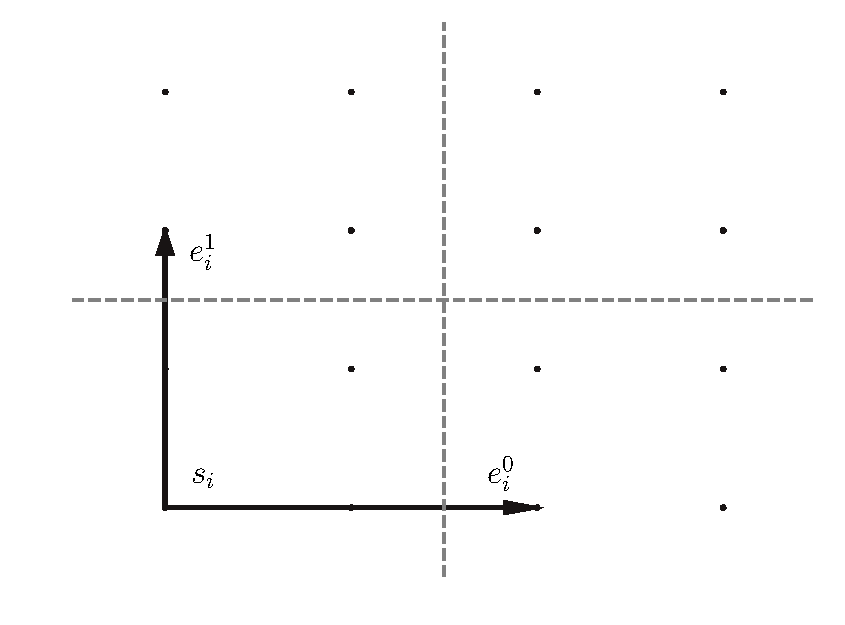
\includegraphics[width=0.6\textwidth]{figures/graphDividing.pdf}
    \caption{One step in the graph dividing algorithm where $l_i = 4$. $e^0_i$ and $e^1_i$ are drawn from site $s_i$. Summed permutations of $\{e^0_i, e^1_i\}$ give the starts for the next boxes. The next iteration of boxes are shown via the dividing dotted lines.}
    \label{fig:graphdividingalgo}
\end{figure}

In order to calculate the box dimension the lattice need to be divided into boxes of decreasing size. A step by step instruction of a graph dividing algorithm is provided below, and an implementation in pseudocode is available in the Appendix at Section \ref{sec:pseudocodeboxdivisionalgo}.

For brevity some abbreviations are introduced.

\begin{equation*}
    \begin{aligned}
        d =& \ \text{dimension} &\quad l_i =& \ \text{side length of the current box}\\
%
        l_0 =& \ \text{side length of the} &\quad e_i^j =& \ \text{vector of length } l_i / 2 \\
%
             & \ \text{smallest box allowed} & & \text{ in the }j\text{'th direction} \\
%
        \text{perm}(v) =& \ \text{All permutations of } v &\quad s_i =& \ \text{starting site of the current box}
    \end{aligned}
\end{equation*}

\begin{enumerate}
    \item If $l_i \geq l_0$, go to 2, else stop.
%
    \item Save all sites in the current box, starting for $s_i$ going $l_i$ in $d$ directions.
%
    \item Find all starting points for new boxes.
%
    \begin{enumerate}[label=(\roman*)]
%
        \item Form the matrix $E = (e_i^0, e_i^1, \  \ldots, e_i^d)^T$
%
        \item For all vectors $v_k$ in perm$(0, 0, \ \ldots , 0)$, perm$(1, 0, \ \ldots , 0)$, \\ \ldots, perm$(1, 1, \ \ldots , 1)$, create the new start $s_k$ as $$s_k = v_k E$$
%
    \end{enumerate}
%
    \item For each start $s_k$:
    \begin{enumerate}[label=(\roman*)]
        \item $s_i = s_k$, $l_i = l_i / 2$
        \item Go to 1.
    \end{enumerate}
%
\end{enumerate}


\chapter{Collider signatures of extra dimensions}\label{ch:ColliderPhenomenology}
\input{chapter5}

\chapter{Summary and conclusions}\label{ch:Summary}
As a first step, the susceptibility of an Ising lattice was examined as can be seen in Fig. (\ref{fig:results_isingsusc}). This is done by measuring the average number of steps taken from each loop in the Worm algorithm. This corresponds to sampling the correlation function, that is related to the susceptibility as $\chi \propto \sum G_{ij}$, where $G_{ij}$ is the correlation function between site $i$ and $j$.


\begin{figure}[h!]
    \centering
        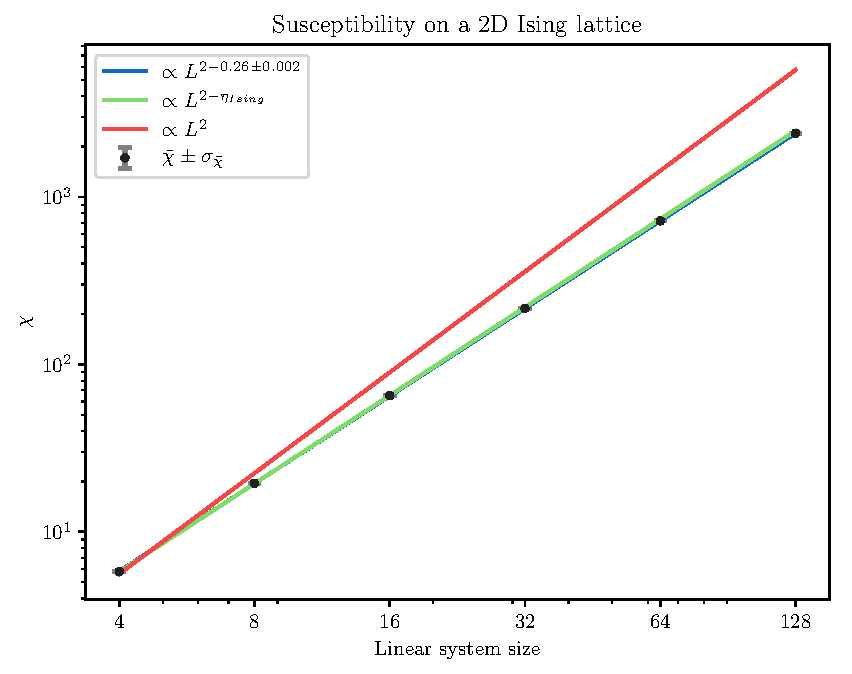
\includegraphics[width=0.8\textwidth]{figures/susceptibility128x128Ising.pdf}
    \caption{Scaling of susceptibility at $T_c$ on an Ising lattice of varying sizes. The measured critical exponent $\eta = 0.262(2)$ is compared to the theoretical value $\eta_{Ising} = 0.25$ \cite{Plischke:EqStatMech}.}
    \label{fig:results_isingsusc}
\end{figure}


\noindent Sampling this correlation function is done for a sequence of different system sizes, $L = 2^n = 4, \ 8, \ 16, \ \ldots, \ 128$, at the critical temperature $T_c = 2 / \ln(1 + \sqrt{2}) \approx 2.27$. According to the known exact solution \cite{Plischke:EqStatMech}, the expected scaling exponent for the Ising susceptibility is $\eta_{Ising} = 0.25$, and is computed here to be $\eta = 0.262(2)$.

Figure (\ref{fig:results_boxdimension}) displays the box dimension of the largest cluster on a $128^3$ Ising cluster. The largest cluster is found by first labeling all clusters with the Hoshen Kopelman algorithm, and then isolating the one with the largest number of links. The graph is then divided into a set of boxes with decreasing sidelength, as showed in the x-axis of Fig. (\ref{fig:results_boxdimension}). The box dimension is then calculated as

\begin{equation}
    d = \lim_{\epsilon \to 0} \frac{\ln N(\epsilon)}{\ln 1 / \epsilon}
\end{equation}

\noindent where $N(\epsilon)$ is the number of boxes needed to cover the cluster. The green line shows the theoretical value for these clusters as $D_H = 1.375$ \cite{Duplantier:GeoHausdorff}, and is computed here to be $D_H = 1.3519(5)$. This illustrates that the achieved accuracy of the box dimension is not very good and a better measure is needed. This is discussed next.

% TODO: Testa loglogplot
\begin{figure}[h!]
    \centering
        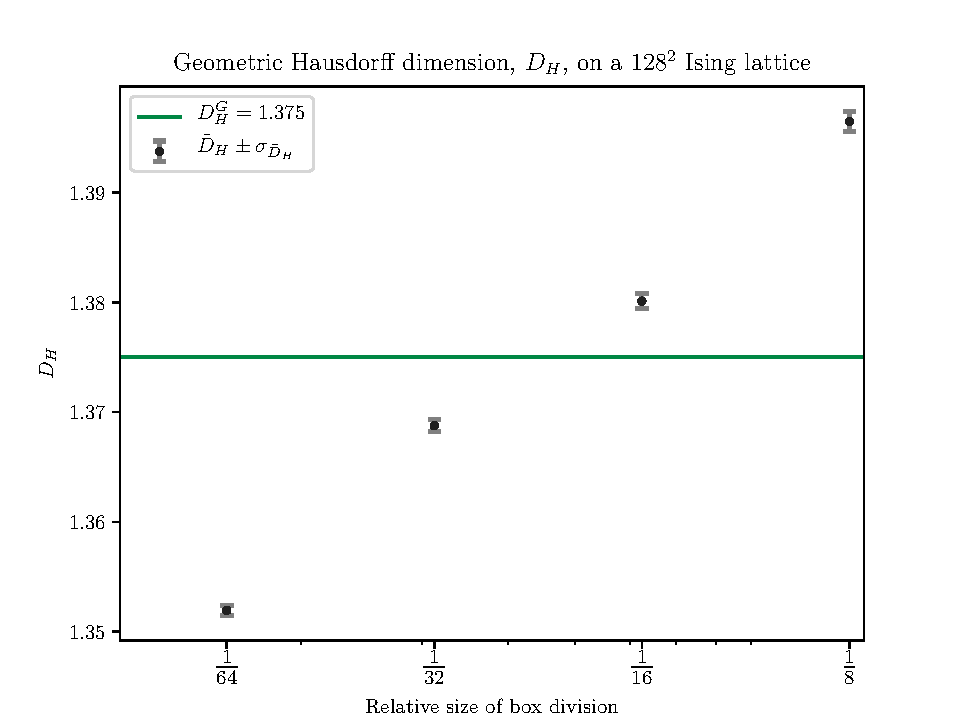
\includegraphics[width=0.8\textwidth]{figures/box_dim_128x128Ising.pdf}
    \caption{Hausdorff dimension of the maximum loop length on a $128^2$ Ising lattice at $T_c$ using the box dimension. The $x$ axis shows the size of one box relative to the side length of the lattice. The green line indicates the theoretical dimension of the geometric Ising cluster, $D_H^G = 1.375$ \cite{Duplantier:GeoHausdorff}. Comparing to the smallest box size as $D_H = 1.3519(5)$.}
    \label{fig:results_boxdimension}
\end{figure}

\newpage

A similar approach is used in Fig. (\ref{fig:results_maxloopdimension}), where the scaling dimension of the largest cluster is examined. The largest cluster in terms of number of links is determined over a sequence of system sizes at $T_c$. This is then fitted to produce a scaling exponent of $D_H = 1.38(2)$ compared to the theoretical value $D_H^G = 1.375$ \cite{Duplantier:GeoHausdorff}. This agrees much better with the theoretical value than the box dimension estimate. 

% TODO: Kolla felstaplar 0.02
\begin{figure}[h!]
    \centering
        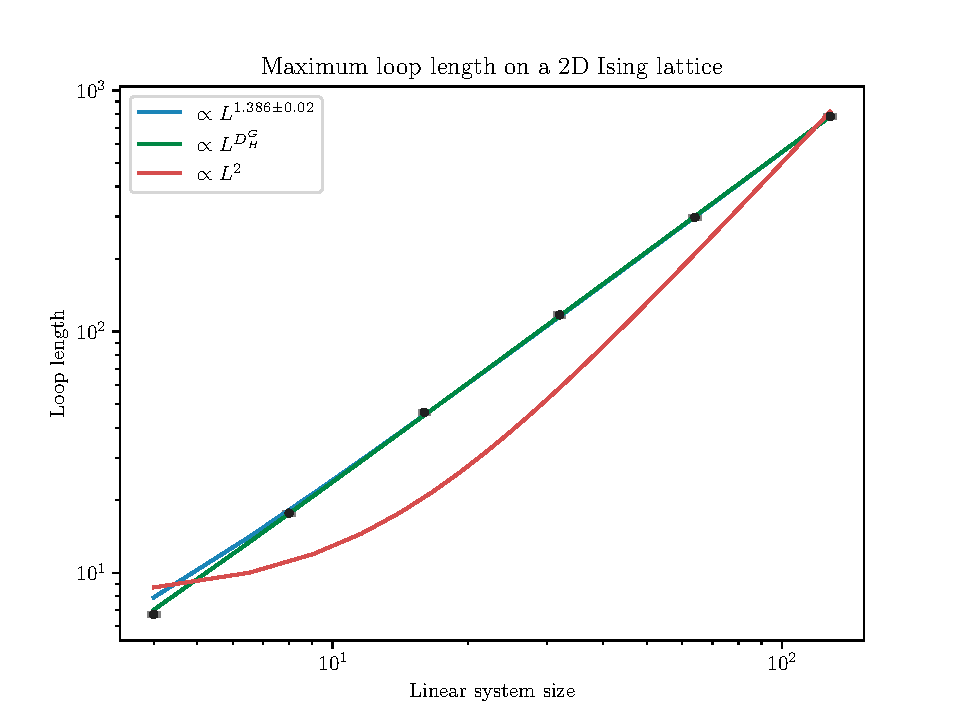
\includegraphics[width=0.8\textwidth]{figures/maximum_loop_length_for_2D_Ising.pdf}
    \caption{Log-log plot of the maximum loop length at $T_c$ on an Ising lattice of varying sizes. The measured scaling factor is $1.38(2)$ compared to the theoretical Hausdorff dimension, $D_H^G = 1.375$ \cite{Duplantier:GeoHausdorff}. Good agreement is obtained.}
    \label{fig:results_maxloopdimension}
\end{figure}

\newpage

Figure (\ref{fig:comparsion_2d_lattice_dimensions}) displays a comparison between the two methods showed in Fig. (\ref{fig:results_boxdimension}-\ref{fig:results_maxloopdimension}) together with the dimensions of random and self avoiding walks. The dimensions computed with the scaling and the box counting method show that the shape of the Ising cluster is similar to that of the self avoiding walk. This can be seen further by examining Figure (\ref{fig:largest_cluster_illu}), where an isolated largest cluster on a $128^2$ Ising lattice is shown.

\begin{figure}[h!]
    \centering
        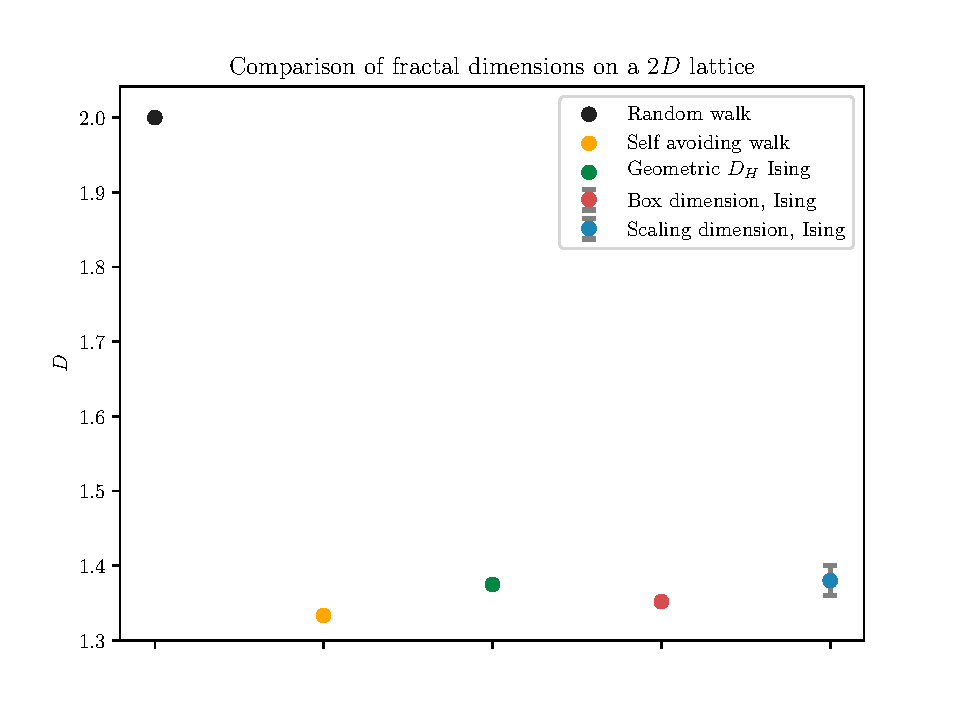
\includegraphics[width=0.8\textwidth]{figures/dimenson_comparison.pdf}
    \caption{Comparison between different algorithms and ways of calculating the fractal dimension on a $2D$ lattice. The random walk has a dimension of $2$, the self avoiding walk has $4/3$ \cite{Vilgis:FlorySAW}. The geometric Hausdorff dimension has an exact value of $1.375$ \cite{Duplantier:GeoHausdorff}. This is then estimated using the worm algorithm and calculated using both the box counting method and the scaling dimension method explained in Sec. \ref{subsec:ScalingDimension}.}
    \label{fig:comparsion_2d_lattice_dimensions}
\end{figure}

\newpage

\noindent The difference between the self avoiding walk and the Ising cluster is that the latter allows the path to cross itself, creating a structure ressembling `twisted loops' as can be seen in Fig. (\ref{fig:largest_cluster_illu}). This might indicate a new type of self avoiding loop, where self crossing is allowed.

\begin{figure}[h!]
    \centering
        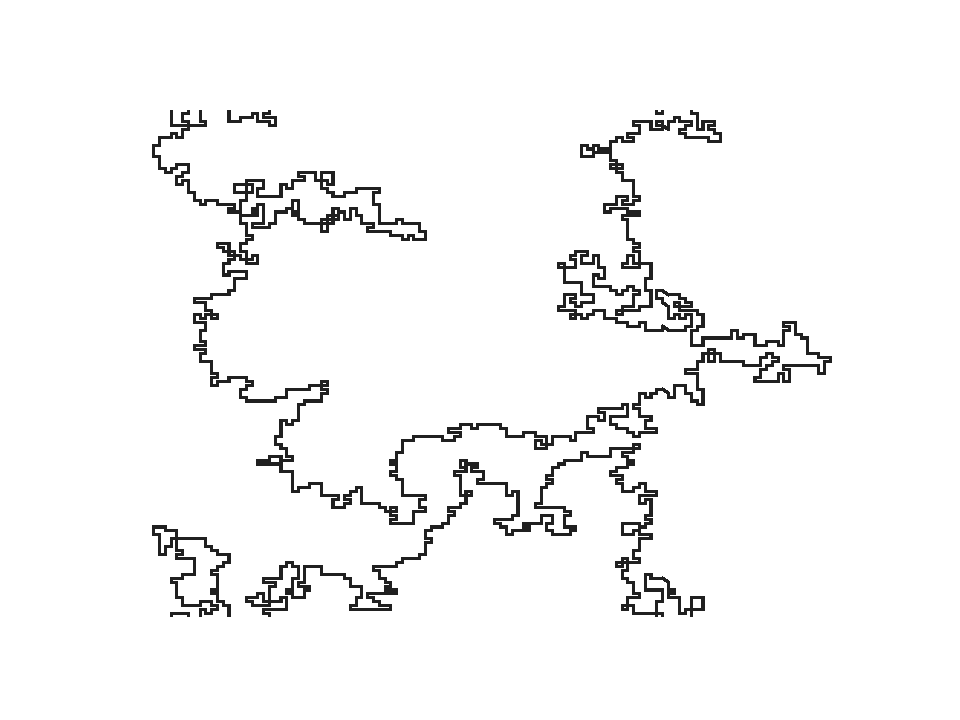
\includegraphics[width=0.8\textwidth]{figures/largest_cluster_testing_nolattice.pdf}
    \caption{Isolated largest cluster on a $128^2$ Ising lattice with periodic boundary conditions.}
    \label{fig:largest_cluster_illu}
\end{figure}

\begin{figure}[h!]
    \centering
        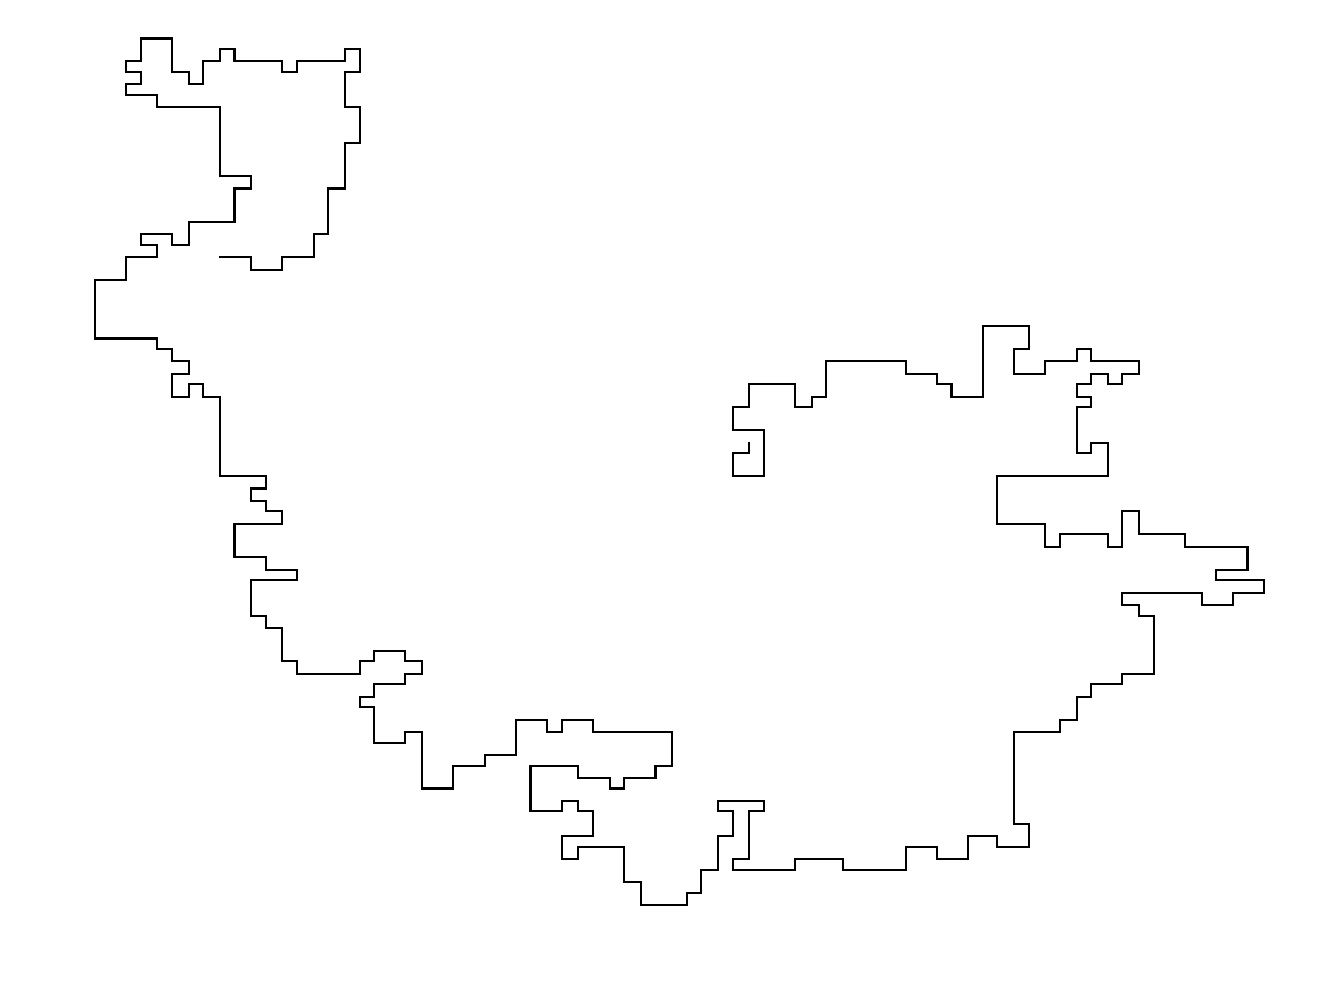
\includegraphics[width=0.8\textwidth]{figures/saw.pdf}
    \caption{Self avoiding walk.}
    \label{fig:result_saw}
\end{figure}

Figure (\ref{fig:result_saw}) displays a purely self avoiding walk. The plot show some similarities to Fig. (\ref{fig:largest_cluster_illu}) in that they both expand away from itself. The self avoiding walk never crosses itself and therefore does not fill the space in its path, resulting in a lower fractal dimension. This can be seen as the coarseness is lower in Fig. (\ref{fig:result_saw}) compared to Fig. (\ref{fig:largest_cluster_illu}).

\newpage

Next, the XY model was examined. To simplify the algorithm, the Villain approximation \cite{Villain:VillainOriginalPaper} was used. This gives a new expression for the energy as

\begin{equation}
    E = \frac{1}{2} \sum_i J^2_i
\label{eq:results_villain_energy}
\end{equation}

\noindent where $J_i$ is the flux associated with site $i$. However, in this approximation, the critical temperature is shifted due to the fact that the acceptance probability is changed by the new expression of the energy. One way of determining the new critical temperature is to measure the superfluid density, as it should fall to zero as the temperature is shifted from above, to below $T_c$. This is done by measuring the winding number, as it relates to the superfluid density as

\begin{equation}
    \langle W^2 \rangle \propto \frac{L}{T} \rho_s
\end{equation}

\noindent for a $3D$ XY lattice. Fig. (\ref{fig:results_windingnumberTc}) show the overall structure of the average winding number squared, plotted for a range of system sizes and temperatures.

\begin{figure}[h!]
    \centering
        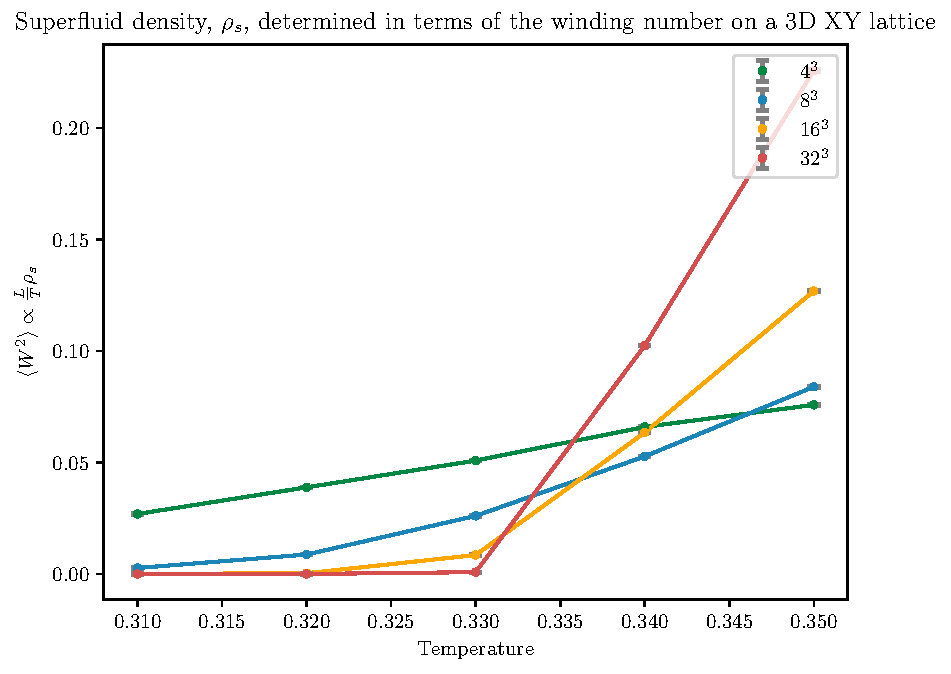
\includegraphics[width=0.8\textwidth]{figures/winding_number_Tc.pdf}
    \caption{Average winding number squared, $\langle W^2 \rangle \propto \rho_s$, plotted on a 3D XY lattice of varying sizes. The overall structure of the average winding number squared as a function of the temperature is shown.}
    \label{fig:results_windingnumberTc}
\end{figure}

\newpage

The intersection between all system sizes of average winding number squared is then determined in Fig. (\ref{fig:results_windingnumberTcZoomed}). The inset, together with the red line shows $T_c = 0.3331(1)$ taken as the weighted average of all intersections with the system sizes as weights. Note here that the temperature in the Villain approximation goes as one over the real temperature \cite{Villain:VillainOriginalPaper}, giving a non-zero superfluid density for high `temperature'.

\begin{figure}[h!]
    \centering
        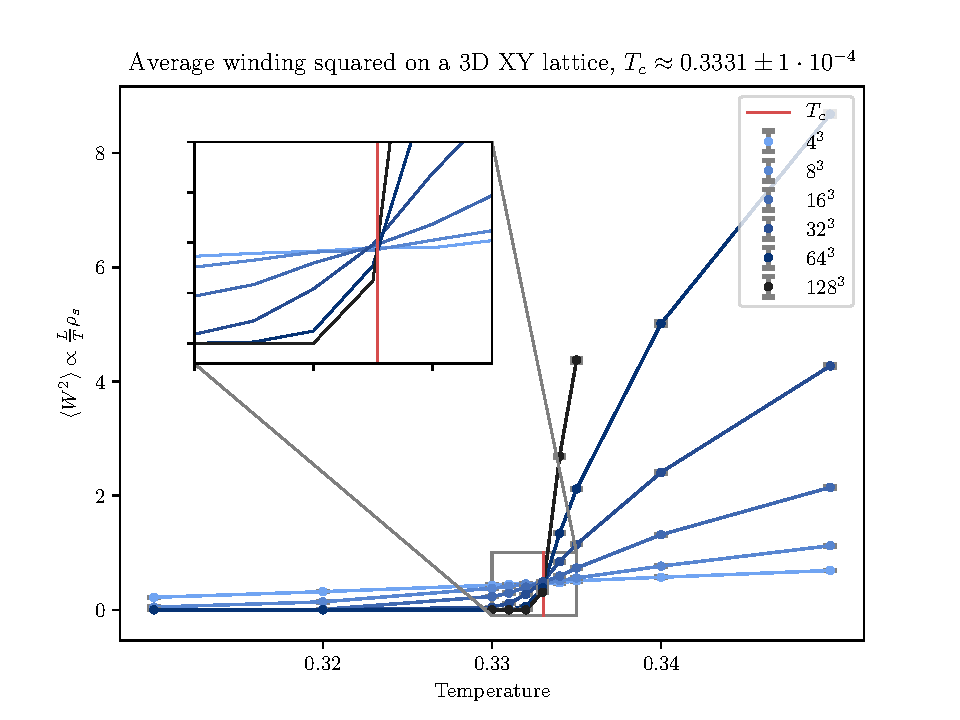
\includegraphics[width=0.8\textwidth]{figures/winding_number_Tc_zoomed.pdf}
    \caption{Average winding number squared, $\langle W^2 \rangle \propto \rho_s$, plotted on a 3D XY lattice of varying sizes. Due to the duality translation the temperature scale is inverted such that $\rho_s \neq 0$ for $T > T_c$, and $T_c$ is translated from $\approx 2.2$ \cite{Gottlob:CritBehaviour3DXY} to $\approx 0.333$ indicated by the intersection. By taking the weighted average of the intersections the critical temperature can be estimated to $T_c = 0.3331(1)$.}
    \label{fig:results_windingnumberTcZoomed}
\end{figure}

\newpage

When the critical temperature has been computed, the box counting method can be applied to the XY system. Figure (\ref{fig:results_boxdimension_xy}) displays the Hausdorff dimension as a function of the relative size of the box. The smallest box indicates the most exact value, $D_H = 1.7747(8)$, and is compared to data from Prokof'ev and Svistunov, $D_H^P = 1.765(2)$ \cite{Prokofev:comment_on_hove_hausdorff_crit_fluct}, and Hove, Mo and Sudbo, $D_H^S = 2.287(2)$  \cite{Hove:hausdorff_crit_fluctuations}. Good agreement with Prokof'ev and Svistunov, while Hove et al.\ deviates. This discrepancy is presumably caused by the different quantity studied by Hove et al., namely vortex loops and phase representations.

% TODO: loglogplot
\begin{figure}[h!]
    \centering
        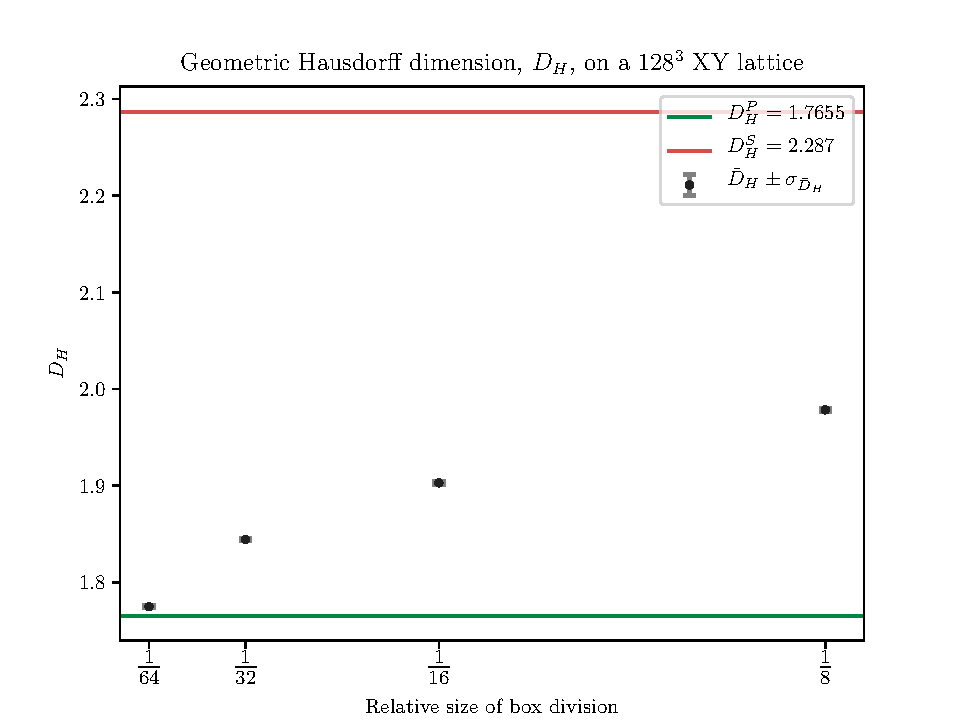
\includegraphics[width=0.8\textwidth]{figures/box_dimension_xy_128x3.pdf}
    \caption{Hausdorff dimension of the maximum loop length on a $128^3$ XY lattice at $T_c$ using the box dimension. The $x$ axis shows the size of one box relative to the side length of the lattice. Assuming that the smallest box size gives the best approximation, the result is $D_H = 1.7747(8)$. This is compared to data from Prokof'evs and Svistunovs paper $D_H^P = 1.765(2)$ \cite{Prokofev:comment_on_hove_hausdorff_crit_fluct} and Hove, Mo and Sudbo's paper $D_H^S = 2.287(2)$ \cite{Hove:hausdorff_crit_fluctuations}.}
    \label{fig:results_boxdimension_xy}
\end{figure}

\newpage

A comparison without the extra data from the larger box sizes is shown in Fig. (\ref{fig:dim_comparison_xy}). The measured dimension from the box counting method closely ressembles that of Prokof'ev and Svistunov.

\begin{figure}[h!]
    \centering
        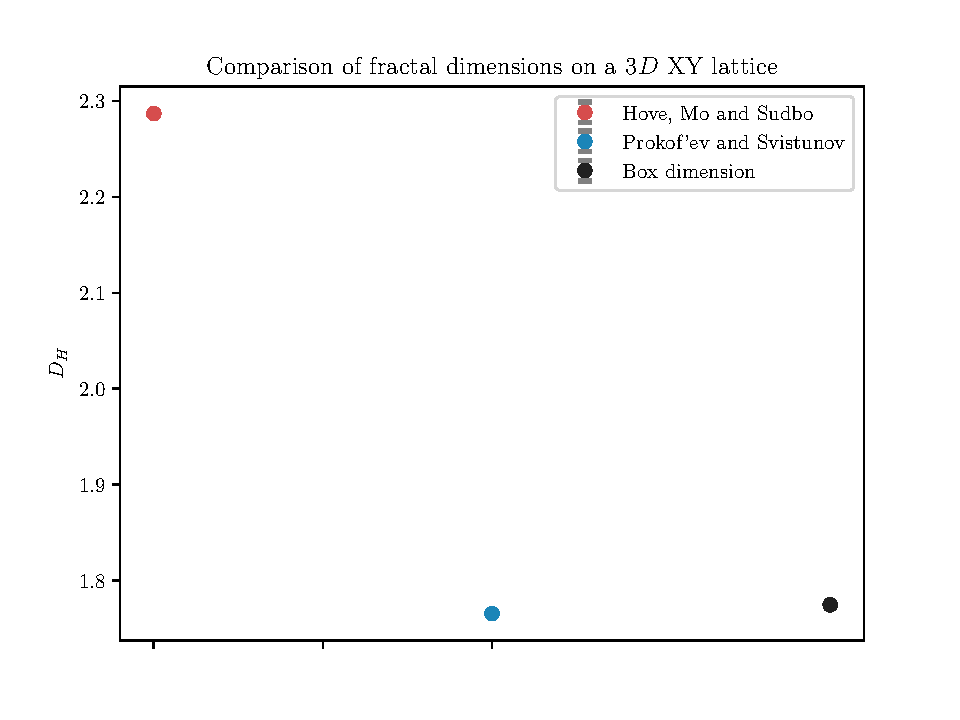
\includegraphics[width=0.8\textwidth]{figures/dimenson_comparison_XY.pdf}
    \caption{Comparison between results from different papers of the Hausdorff dimension of the maximum loop length on a XY lattice at $T_c$. The result from this thesis is labeled `box dimension' and yields the result $D_H = 1.7747(8)$. This is compared to data from Prokof'evs and Svistunovs paper $D_H^P = 1.7655 \pm 2 \cdot 10^{-3}$ \cite{Prokofev:comment_on_hove_hausdorff_crit_fluct} and Hove, Mo and Sudbo's paper $D_H^S = 2.287 \pm 2 \cdot 10^{-3}$ \cite{Hove:hausdorff_crit_fluctuations}.}
    \label{fig:dim_comparison_xy}
\end{figure}

\newpage

Finally, the total energy of the XY lattice is plotted for a sequence of system sizes at $T_c$. The total energy is calculated in the Villain approximation as shown in Eq. (\ref{eq:results_villain_energy}). This scaling coefficient of the energy here is $2.91(9)$, and is therefore close to scaling as the spatial dimension of the system. This is expected since 

\begin{equation}
    E = L^d ( a t^{1 - \alpha} + b ) \propto L^d, \ \text{at $T = T_c$}
\end{equation}

\noindent where $t = T - T_c$, and $a$ and $b$ are some unknown constants.

\begin{figure}[h!]
    \centering
        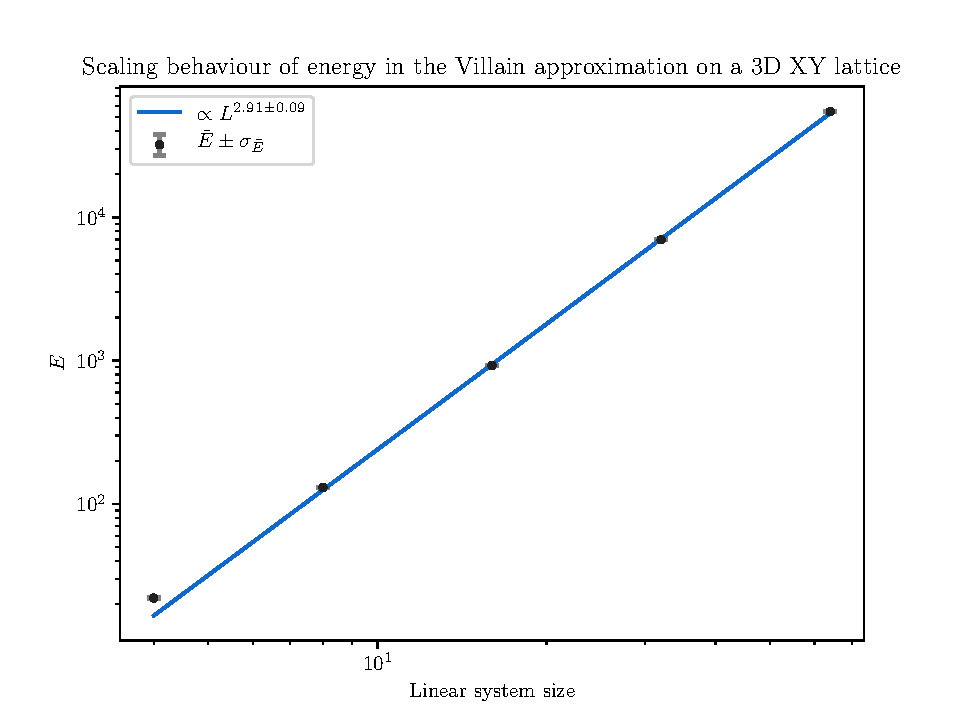
\includegraphics[width=0.8\textwidth]{figures/energy_scaling_xy.pdf}
    \caption{Log-log plot of the energy at $T_c$ on an 3D XY lattice of varying sizes. The measured scaling factor is $2.91(9)$. The energy in the Villain approximation is proportional to the sum of the squares of flux flowing through the lattice.}
    \label{fig:results_energyxy}
\end{figure}




% This starts the appendices.
%\appendix

%\chapter{Appendix about something}
%\input{appendix}

\addcontentsline{toc}{chapter}{Bibliography}
\bibliographystyle{thesis_bib_style}
\bibliography{references}

\part{Scientific papers}

\input{prepapers}

\end{document}





